\documentclass[11pt, a4paper]{article}
\usepackage{amsmath}
\usepackage{amssymb}
\usepackage{amsthm}
\usepackage{epsfig}
\usepackage[margin=1in]{geometry}
\usepackage{enumitem}
% \usepackage{enumerate}
\usepackage{graphicx}
\usepackage{multirow} %For merging multiple rows in a table object
\usepackage{booktabs}
%%%%%%%%%% Package for Highlight         %%%%%%%
\usepackage[usenames, dvipsnames]{xcolor}


%%%%%%%%% Reference Style Here %%%%%%%%%%%%%%%%
\usepackage[utf8]{inputenc}
\usepackage{csquotes}
\usepackage[english]{babel}
\usepackage[backend=biber,style=numeric,sorting=none]{biblatex}
\addbibresource{Reference.bib}

%%%%%%%%%%%%%%%%%%%%%%%%%%%%%%%%%%%%%%%%%%%%%%%%
\usepackage{tikz}
\usetikzlibrary{automata, positioning}
\usepackage{caption}
\usepackage{mathtools}
\usepackage{algorithm}
\usepackage{algorithmic}
\usepackage{todonotes}
\usepackage{times}
\usepackage{pdfpages}
\usepackage{mathtools}
%\usepackage[]{algorithm2e}

\usepackage{lipsum} % paragraph spacing
\usepackage{titlesec} % paragraph spacing
\usepackage{comment}
%%%%%%%%%%% CHINESE TYPING  %%%%%%%%%%%%
\usepackage{CJK} 
% How to use: 
% \begin{CJK}{UTF8}{} 
% \end{CJK}
%%%%%%%%%%%%%%%%%%%%%%%%%%%%%%%%%%%%%%%%%%%

%%%%%%%%%%%%%%%%%%%%%%%%%%
% 3 Columns & landscape	 %
%%%%%%%%%%%%%%%%%%%%%%%%%%
%\usepackage{multicol}
%\usepackage{pdflscape}

% For writing code:
\usepackage{fancyvrb}
\DefineVerbatimEnvironment{code}{Verbatim}{fontsize=\small}
\def\showvrb#1{%
	\texttt{\detokenize{#1}}%
}

\linespread{1.1}
\setlength{\parindent}{0pt} % Sets the indent length to 0
\setlength{\parskip}{0pt plus 1pt minus 1pt} % paragraph vertical distance

\everymath{\displaystyle} % displays inline math as displaymath

\hyphenpenalty=10000 % force no hyphenation



\begin{comment}
%%%%%%%%%%%%%%%%%%%%%%%%%%%%%%%%%
% ONLY RECOMMENDED FOR 3 COLUMN %
%%%%%%%%%%%%%%%%%%%%%%%%%%%%%%%%%%%%%%%%%%%%%%%%%%%%%%%%%%%%%%%%%%%%%

\setlist[itemize]{noitemsep, topsep=0pt, leftmargin=0.2in} % compacts lists with no item separation,indent from the left side = 0.2
\titlespacing\section{1pt}{5pt plus 4pt minus 2pt}{2pt plus 2pt minus 2pt}%paragraph spacing
\titlespacing\subsection{0pt}{5pt plus 4pt minus 2pt}{2pt plus 2pt minus 2pt}%paragraph spacing
\titlespacing\subsubsection{0pt}{5pt plus 4pt minus 2pt}{2pt plus 2pt minus 2pt}%paragraph spacing
\end{comment}


%%%%%%%%%%%%%%%% Normally use this! %%%%%%%%%%%%%%%%%%%%%%%%%%%%%%%%%%%%%%%%%%%%%%%%%%%%
%
\setlist[itemize]{noitemsep, topsep=3pt} % compacts lists with no item separation    %%%
%
%
%%%%%%%%%%%%%%%%%%%%%%%%%%%%%%%%%%%%%%%%%%%%%%%%%%%%%%%%%%%%%%%%%%%%%%%%%%%%%%%%%%%%%%%%


\title{Performance Gap}
\author{Ying He}

%%%%%%%%%%%%%%%%%%%%%%%%%%%%%%%
%   Commonly used theorems    %
%%%%%%%%%%%%%%%%%%%%%%%%%%%%%%%

% Use roman for text - numbering follows onwards
\theoremstyle{definition}
\newtheorem{defn}{Definition}[section]
\newtheorem{them}{Theorem}[section]
\newtheorem{lem}{Lemma}[them]
\newtheorem{prop}[them]{Proposition}
\newtheorem{corr}[them]{Corollary}
\newtheorem{corrr}{Corollary}[them] %for consistency issues
% examples follow different numbering
\newtheorem{eg}{Example}[section]
\newtheorem{egg}[them]{Example}
\newtheorem*{themf}{Theorem 5.0}
\newtheorem*{themm}{Theorem}
\newtheorem{question}{Question}

%%%%%%%%%%%%%
% Shortcuts %
%%%%%%%%%%%%%

\newcommand{\Q}{\mathbb{Q}}
\newcommand{\C}{\mathbb{C}}
\newcommand{\F}{\mathbb{F}}
\newcommand{\R}{\mathbb{R}}
\newcommand{\Z}{\mathbb{Z}}
\newcommand{\N}{\mathbb{N}}
\newcommand{\D}{\mathbb{D}}

\newcommand{\mcC}{\mathcal{C}}
\newcommand{\mcN}{\mathcal{N}}
\newcommand{\mcE}{\mathcal{E}}
\newcommand{\mcP}{\mathcal{P}}
\newcommand{\mcF}{\mathcal{F}}
\newcommand{\mcS}{\mathcal{S}}
\newcommand{\mcA}{\mathcal{A}}
\newcommand{\mcB}{\mathcal{B}}
\newcommand{\mcX}{\mathcal{X}}
\newcommand{\mcL}{\mathcal{L}}
\newcommand{\mcH}{\mathcal{H}}
\newcommand{\mcl}{\mathcal{l}}

\newcommand{\bfe}{\mathbf{e}}
\newcommand{\mbf}{\mathbf}

\newcommand{\ran}{\mbox{Ran}}

\newcommand{\al}{\alpha}
\newcommand{\s}{\sigma}
\newcommand{\ep}{\epsilon}
\newcommand{\dl}{\delta}
\newcommand{\sg}{\sigma}

\newcommand{\bs}{\backslash}
\newcommand{\n}{\\}
\newcommand{\ol}{\overline}
%\newcommand{\bb}{\textbf} %Bold front
%\newcommand{\ul}{\underline} %underline

\newcommand{\ltlU}{\textsf{ \bfseries UNTIL }}
\newcommand{\ltlF}{\textsf{\bfseries F }}
\newcommand{\ltlG}{\textsf{\bfseries G }}
\newcommand{\ltlX}{\textsf{\bfseries X }}
\newcommand{\ltlA}{\textsf{\bfseries A }}
\newcommand{\ltlE}{\textsf{\bfseries E }}

%%%%%%%%%%%%%%%%%%%%%%%%%
% Standard big brackets %
%%%%%%%%%%%%%%%%%%%%%%%%%

\newcommand{\floor}[1]{\left\lfloor{#1}\right\rfloor}
\newcommand{\ceil}[1]{\left\lceil{#1}\right\rceil}
\newcommand{\bbA}[1]{\left({#1}\right)}
\newcommand{\bbB}[1]{\left[{#1}\right]}
\newcommand{\bbC}[1]{\left\{{#1}\right\}}



%%%%%%%%%%%%%%%%%
%  MATRIX       %
%%%%%%%%%%%%%%%%%
\newcommand{\matxx}[9]{\begin{pmatrix} #1 & #2 & #3 \\ #4 & #5 & #6 \\ #7 & #8 & #9 \end{pmatrix}}
\newcommand{\matx}[4]{\begin{pmatrix} #1 & #2 \\ #3 & #4 \end{pmatrix}}
%example
%    $\matx{1}{2}{3}{4}{5}{6}{7}{8}{9}$

%%%%%%%%%%%%%%%%

%%%%%%%%%%%%%%%%%%%%%%%%%%%%%
% Highlight color
%%%%%%%%%%%%%%%%%%%%%%%%%%%

\newcommand{\hgy}{\colorbox{GreenYellow}} % Light Green
\newcommand{\hyg}{\colorbox{YellowGreen}} % another Light Green
\newcommand{\hlb}{\colorbox{SkyBlue}} % light blue
\newcommand{\hpink}{\colorbox{pink}} % Light pink
\newcommand{\hor}{\colorbox{orange}} % Orange
\newcommand{\hlor}{\colorbox{Apricot}} % Light Orange




%%%%%%%%%%%%%%%% SET Graphics Path %%%%%%%%%%%%%%
\graphicspath{{./Figure/}}




%%%%%%%%%%%%%%%%%%
% Start Document %
%%%%%%%%%%%%%%%%%%
\setlength{\marginparwidth}{2cm}
\begin{document}
\begin{comment}
	\begin{landscape}
	\begin{multicols*}{3}
\end{comment}

\begin{comment}
\textbf{abcdefg}



%\tableofcontents


\hlor{abcd}

\[\matx{1}{2}{3}{4}\] al;dfjajfa

woyaozaizhedazi $\matx{1}{2}{3}{4}$



\[\alpha \cdot \beta \]
123456789/*
\end{comment}
\maketitle

\newpage
\tableofcontents

\newpage
\section{Abstract}
This thesis aims to reduce the deviation between calculated and measured heating demands and find the short-comings in SIA 380/1 calculation method. A residential building and an office building are accurately modeled and calculated using EnergyPlus and SIA 180 standard. Both buildings are firstly calibrated based on historical annual heating demand and hourly indoor temperature, then several key building parameters are changed into different values. Based on a large number of simulations, the result indicated that the most influential parameters in simulation are key area temperature heating set points, external wall solar absorptance, infiltration and lighting schedule. In order to reduce the performance gap, it is recommended to create an accurate building envelope and apply accurate outdoor environment. Therefore, an update to SIA standard weather data is also recommended.
\cite{FREI2017421}

\newpage
\section{Introduction}
	
		Building simulation are widely used for different purposes such as to benchmark buildings or to evaluate energy demands and indoor thermal comforts. However, due to a number of factors, there are deviations between calculated  and measurement values, which is called \textbf{performance gap}. Previous studies which used a standardized method \textbf{SIA 180/1} to calculate the heating demand of several buildings observed considerably large performance gaps in uninsulated buildings \cite{SIAPreviousreport}. It is believed that part of the problem come from a non-accurate calculation method or non-realistic assumptions to some building parameters and outdoor environment \cite{SIAPreviousreport}. \\
	
	
		Therefore, the purpose of this thesis is to find out the main causes of the performance gap in uninsulated buildings, as well as the most influential factors in building simulation. In addition, this thesis also aim to investigate how the resulting energy demand variations affect the performance gap.\\

	
		Two uninsulated buildings, one residential and one office buildings, are carefully modeled and analyzed using different approaches including SIA 180/1 calculation and EnergyPlus simulation. The buildings is firstly calibrated to match the historical measurement, then building parameters are modified and the most influential factors can be discovered.

			\begin{figure}[h!]
			\centering
			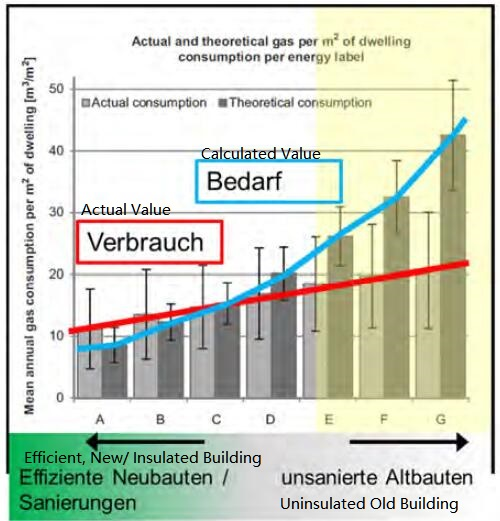
\includegraphics[scale=0.65]{Figure/SIA380Issue.jpg}
			\caption{SIA380/1 Calculation Performance Gap Indicator \cite{SIAPreviousreport}}
			\label{fig:SIA380PG}
			\end{figure}


\newpage		
\section{Literature Review}

	Over the past years, there are a large number of research about building energy performance gap (BEPG). Performance gap can cause problems in energy management system. However, the root cause of this gap is not clearly identified, and the gap can't be effectively managed and eliminated \cite{FREI2017421}.
	According to a recent review of building energy performance gap by Zou and Xu et.al, most of them would contain one or more of the following 5 elements: (1) building type, which can be classified as residential and non-residential, or even more specific types such as single-family house, multi-family house, office building, commercial building, hospital, prison, etc; (2) strategies for closing performance gap, which focus about design concept, technology and method, and "soft" measures; (3) building life cycle, which analyses the cause of performance gap in different stages of a building; (4) energy-related stakeholders, whose behavior would affect the performance gap; (5) the influence factors or building parameters that would cause or affect the performance gap \cite{FREI2017421,ZOU2018165}. Consider the objective of this thesis, the focus is on these following topics.
	
	\subsection{Formation of Performance Gap}
		Most causes of performance gap can be grouped into 3 categories base on the stages in the building life-cycle. They are design and simulation problems, misbehavior of contractors and misbehavior of building users \cite{userevaluations,NIU2016275}.
		
		\subsubsection{Design and simulation problem}
		Firstly, in most cases, building designers are account for the wrong doings in design and simulation processes. These include wrong assumptions and predictions about their design such as inaccurate building unheated area's temperature, wrong representation of user behavior, and wrong forecast of outdoor environment \cite{HOFFMANN201731,NIU2016275}. Also, it is difficult to predict the future environment such as climate, weather, and solar activities, which factors can lead to huge performance gaps \cite{DIAZ2017393,doi:10.1080/19401493.2012.718797}. For example, rainfall would greatly increase the heat convection coefficient of building facade surface, and therefore increase heat exchange rate through the building envelope \cite{DIAZ2017393}. In addition, the actual thermal performance of building materials subject from different factors and are usually perform worse than how they should in lab environments. Therefore, designers usually overestimate the actual performance of technology and apply inappropriate assumptions about user behaviors \cite{DEWILDE201440}. 

		\subsubsection{Contractors}
		Secondly, contractors are mainly account for performance gaps caused by low quality constructions. Poor building quality and poor workmanship will usually reduce the thermal performance and therefore require more energy to maintain indoor comfort. Additionally, performance gap can be caused by contractors when they use improper construction techniques and when they are unable to discover hidden problems due to time and budget constraints \cite{DEWILDE201440}.In some cases, these problems would lead to huge building parameter deviations and therefore higher energy consumption than the design value \cite{FREI2017421,DEWILDE201440}. 

		\subsubsection{User behaviors}
		Lastly, as the last and main stage of building's life-cycle, different behaviors of building users are also important sources of performance gap \cite{ZOU2018165}. These behaviors, either deliberate or unconscious, are usually not the optimum ways to operate a building. Building owners or occupants have specific behaviors due to their social and personal characteristics, attitude, experience, and thermal comfort standard \cite{userevaluations,LAWRENCE2016651}. For example, users may leave unnecessary appliance on without notice or open the windows when heatings or cooling system is operating \cite{FREI2017421}.

	\subsection{Strategies For Closing Performance Gap} 
		When the causes of performance gap are found out, strategies for closing the gap can also be developed. These strategies are grouped into 3 categories, which is, namely, design concept, technology and methods, and "soft" measures \cite{ZOU2018165}.

		\subsubsection{Design Concept}
			\textit{Passive design} is thought to be able to eliminate or decrease the impact of user behavior on energy consumption. Its philosophy is that if a building is designed in a way that no active equipment is needed, user behaviors would not influence the passive mechanism \cite{BLIGHT2013183,NORFORD1994121}. However, this approach has high construction quality requirements and can only have positive effects when both building designers and the occupants fully understand the building energy system. If building designers have inaccurate information about occupants, or building constructors don't have the capability to construct the building according to the specifications, or if the occupants do not fully understand the building system, passive design approach can only have adverse impacts \cite{ZOU2018165}.\\

			\textit{Active design}, on the other hand, use building automation system to improve occupants' thermal comfort and hopefully reduce the chance of wrong operations by occupants. Same as passive design, this design approach also require high quality equipment and construction team, and a comprehensive understanding of buildings and occupant behaviors to function well \cite{DEWILDE201440}.\\

			\textit{Human-in-the-loop} is another approach that requires human interaction \cite{karwowski2001international}. As information is a critical factor in building energy, the more comprehensive and accurate the obtained data, the more precise the result would become \cite{NIU2016275}. Therefore, in order to improve the accuracy of "human-in-the-loop design", is of importance to collect accurate data. There have been research which used advanced technology such as genetic algorithm, machine learning, VR and AR to collect building data for simulations and calculations \cite{karwowski2001international}. The limitations of this approach would be the difficulty to collect comprehensive human information, and there is an uncertainty of occupants behaviors and different occupants may influence each other \cite{masoso2010dark}.

		\subsubsection{Technology and methods (T\&M)}

			It is believed that using more advanced and innovative technologies and calculation methods would help closing the performance gap \cite{ZOU2018165}. Previous research has grouped most technologies and methods into 4 categories, namely T\&M for calculating energy consumption, T\&M for energy related data collection and analysis, T\&M for occupant behavior modeling and simulation and T\&M for energy system controlling \cite{ZOU2018165}.\\

			\textit{T\&M for calculating energy consumption}\\

			\textit{T\&M for calculating energy consumption} can be further divided into \textit{Black box} methods, \textit{Grey box} methods, and \textit{White box} methods. A black box method, such as genetic algorithm and artificial neural networks, calculates energy consumption without physical knowledge. The white box method, such as \textit{EnergyPlus, DOE-2, Ecotect} calculation engines, calculates energy consumption base on thermodynamic behavior of the building and its occupants \cite{li2014methods,xu2007optimal}. The grey box method is a combination of the black and white box method, in hope of eliminating the limitations of both methods \cite{ZOU2018165}.\\

			\textit{T\&M for data collection and analysis}\\

			\textit{T\&M for data collection and analysis} focuses on obtaining and utilizing the occupant behavior and building operation information \cite{ZOU2018165}. Similarly, T\&M for data collection and analysis can be divided into two approaches, namely \textit{post occupancy} data collection and \textit{pre-occupancy} data collection \cite{ZOU2018165}. \textit{Post-occupancy data collection} is the traditional and most commonly used data collecting approach which use different sensors and monitors to record occupants' activities as shown in Figure \ref{fig:Energy_DataCollection} below. However, since all buildings are more or less different from each other, post-occupancy data collection would not provide a customized and future-oriented prediction of a newly designed building, neither would it explain the reasons behind certain occupant behaviors \cite{NIU2016275}.\\

			To overcome this limitation, \textit{pre-occupancy data collection} is developed to collect virtual occupancy behavior data based on VR or BIM building models. By this approach, customized occupancy data can be collected and designers can also improve the building design base on the collected virtual occupancy data. However, this method is not flawless, as the virtual occupancy behavior would likely be different from the actual behaviors in the real buildings.\\


			\begin{figure}[h!]
			\centering
			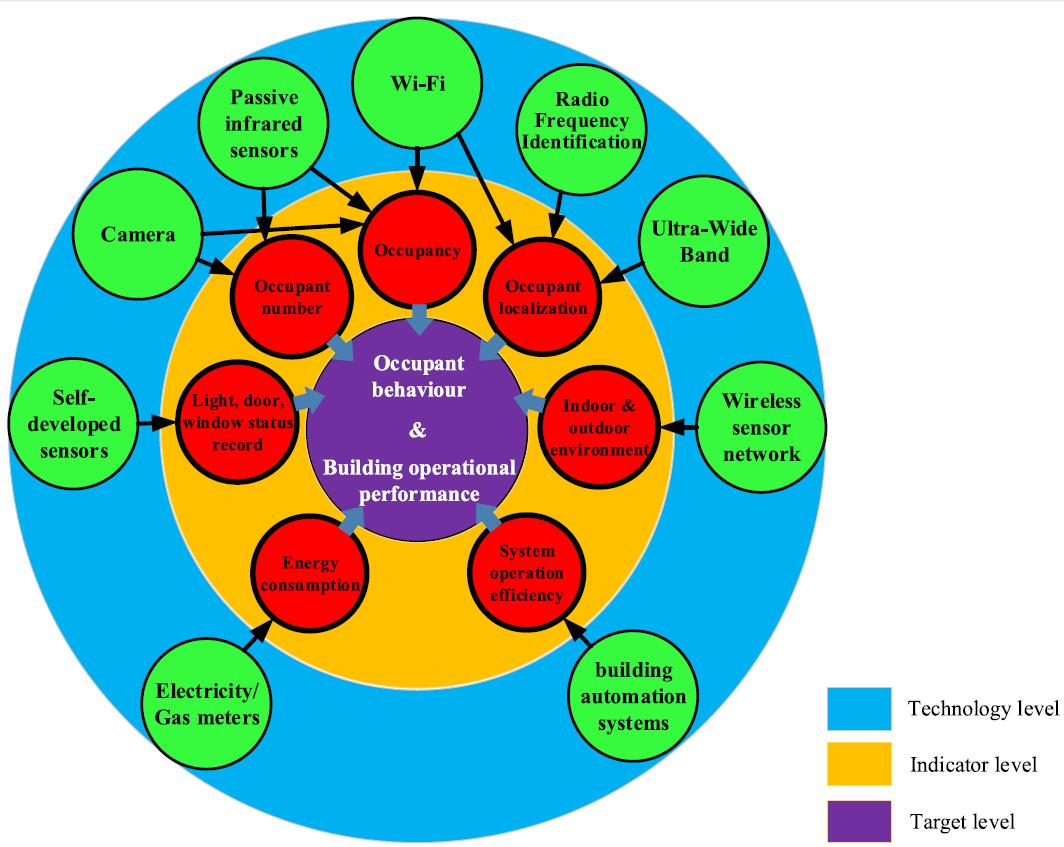
\includegraphics[scale=0.5]{Energy-relatedData.jpg}
			\caption{Technology and method for energy-related data collection \cite{jia2017occupancy}}
			\label{fig:Energy_DataCollection}
			\end{figure}

			\begin{figure}[h!]
			\centering
			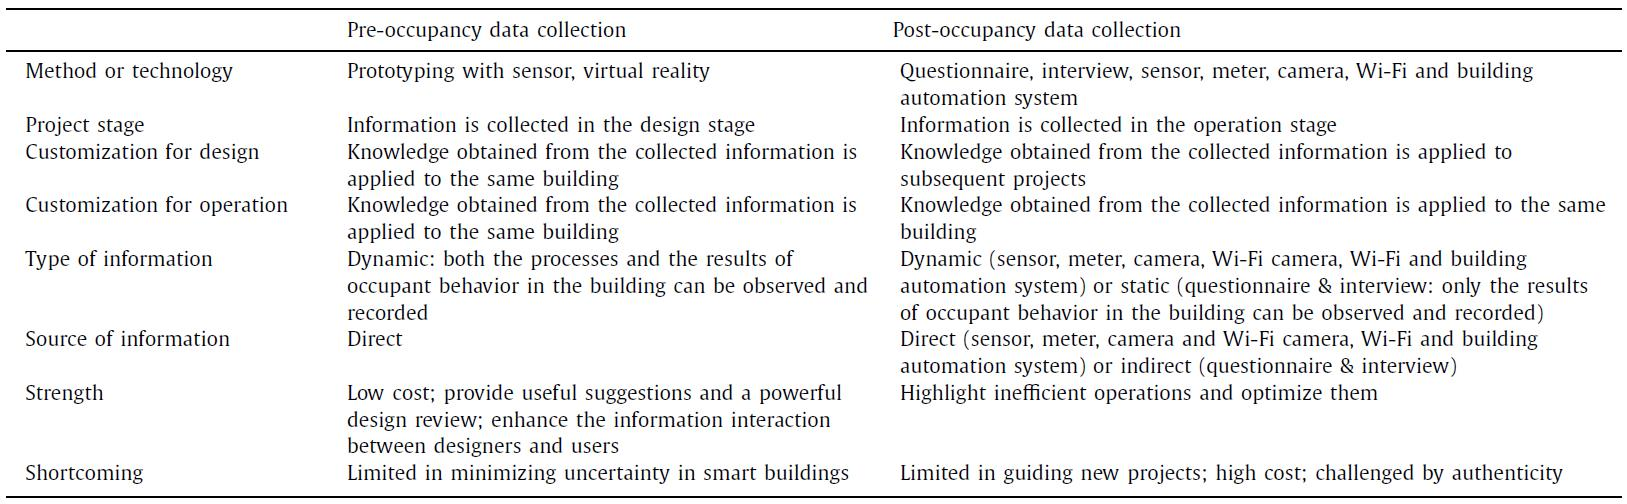
\includegraphics[scale=0.4]{Table1.jpg}
			\caption{Comparison of pre-occupancy data collection and post-occupancy data collection \cite{ZOU2018165}}
			\label{fig:technology1}
			\end{figure}

			\textit{Statistical analysis} is mostly used to develop a numerical relationship among energy consumption, outdoor environment, indoor environment and comfort, occupant behavior and other information using statistical tests, regression analysis and curve fitting \cite{ZOU2018165}. Previous research also show that the above mentioned data collection approaches would be slow and expensive, and the collected data volume is massive and unstructured \cite{liang2016occupancy}.\\

			In order to process this massive amount of data, \textit{Data mining} would be a good technology to structure the collected data and find out the unknown correlations between different data sets. Currently, data mining is used to analyze building energy consumption data and occupancy/occupant behavior data \cite{xiao2014data}.\\

			\textit{T\&M for occupant behavior modeling and simulation}\\

				As building occupants are capable to greatly alter the building indoor environment, it is of importance to know how exactly did they operate the building when a building is subjected to energy analysis or building simulations. However, obtaining an exact set of occupant activity record through the simulation period is hardly possible for most cases. Therefore, some technologies and methods are developed to generate a reasonable set of occupant behavior. \textit{T\&M for occupant behavior modeling and simulation} are mainly two groups, namely \textit{agent-based modeling (ABM)} and \textit{stochastic process modeling} \cite{ZOU2018165}.\\


				\textit{Agent-based modeling (ABM)}\\
				\textit{Agent-based modeling (ABM)} simulates the actions and interaction of agents, such as individual, group or equipment, and investigate how they interact with the whole system \cite{jia2017occupancy}. Some previous studies have used ABM to address the interrelation between different occupants, or to simulate user-defined social constraints from other occupants on an agent's certain behavior. The advantage of ABM is its potential capability to integrate with energy simulation program and its capability to deal with interactions and uncertainties \cite{ZOU2018165}. However, the limitation of ABM is not negligible. Currently, ABM are more dependent on assumptions rather than actual data, and it is difficult to verify a model based on ABM \cite{ZOU2018165,jia2017occupancy}. \\


				\textit{Stochastic process modeling}\\
					As the occupant behavior is more or less random, \textit{stochastic modeling} can be widely used in many researches involing estimating probability distributions of occupant behavior. In most cases, stochastic process modeling approach focus on relatively long-term occupancy prediction or classification instead of a certain behavior at a certain time \cite{ZOU2018165}.
					In this thesis, stochastic process modeling approach based on SIA standards is used in the dynamic energy analysis part, the detailed parameters can be found in chapter methodology.\\


			\textit{T\&M for building mechanical system controlling}\\

				\textit{T\&M for energy system controlling} aims at reducing building energy consumption without sacrificing the occupants' thermal comfort, and can be devided by three groups: \textit{intelligent HVAC system, artificial lighting} and \textit{occupancy-based control system} \cite{ZOU2018165,hong2015review}. The limitation for T\&M for building automatic control would be it relies heavily on controlling algorithms and the accuracy of sensoring equipments. Therefore, a mal-functioning sensor group would paralise the control system.

		\subsubsection{"Soft" Measures}
			Apart from several policy measures, one of the \textit{"soft measures"} would be to develope a more comprehensive and reliable benchmarking and standard tools to improve building energy performance. Some of these guildlines or benchmark standards are National Australia Building Environment Rating Standard (NA BERS), Australia's Green Star, European Union Passive House, UK's Building Research Establishment Environment Assessment Method (BREEAM), Swiss Minergie, US's Leadership in ENergy and Environmental Design (LEED) and Energy Star \cite{ZOU2018165}. However, these benchmark standards rely heavily on predicted building comfort and energy consumption, while the actual energy consumption is usually far from the calculated values \cite{tuohy2015closing}. As there are many designers use standard benchmark calculation tool as their design basis, developing a more reliable calculation method would be a good approach to improve the problem.


	\subsection{Selection of Simulation Tools}
		Crawley and Hand et.al provided a comprehensive review on currently in-use building energy simulation tools back in 2008, and it include a brief review of EnergyPlus 1.2.2 and its basis building simulation tools \cite{crawley2008contrasting}. As EnergyPlus is compatible with building modeling software \textit{DesignBuilder}, it is more convenient to use it in this thesis comparing to other simulation tools. Additionally, as EnergyPlus is based on the features and capabilities of BLAST and DOE-2, these two tools are also briefly reviewed \cite{crawley2008contrasting}. Although the reviewed EnergyPlus version is more than 10 years old, it is believed that the bone structure of the tool remains the same till today.\\

		\textbf{Building BLAST}\\
			The BLAST system predicts building energy consumption, building energy system performance and building costs \cite{crawley2008contrasting}. It contains three major subprograms: Space Loads Prediction, Air System Simulation, and Central Plant. \textit{Space Loads Prediction} computes hourly space loads based on the given hourly weather data, building construction properties and operation details. It uses a radiant, convective, and conductive heat balance for all surfaces and a heat balance of indoor air \cite{crawley2008contrasting}. The energy balance equations include heat transmission, solar loads, internal heat gains, air infiltration loads, and temperature control strategy used to manipulate the indoor temperature. BLAST can be used on new or existing buildings of almost any type and shape \cite{crawley2008contrasting}.\\

		\textbf{DOE-2.1E}\\
			DOE-2 predicts hourly energy consumption and energy cost for a building based on the given weather information, building geometry, HVAC description, and utility cost. DOE-2 has one subprogram to translate input (BDL Processor), and four simulation subprograms namely \textit{Loads, Systems, Plant, and ECON (Economics)}.\\
			\textit{Loads, Systems and Plant} are executed in sequence, with the output of the predecessor become the input of the next program in sequence. The output then becomes the input to \textit{Economics} \cite{crawley2008contrasting}. Each of the simulation subprograms can also generate printable reports of the results of its calculations.\\
			DOE-2 has been used extensively for more than 35 years for both building design studeis, retrofit analysis, and for developing and testing building energy standards \cite{crawley2008contrasting}.\\
		

		\textbf{EnergyPlus}\\
			\textit{EnergyPlus} is a modular and structured code based calculation engine. As mentioned above, it is based on the most popular features and functions of BLAST and DOE-2 and it is a more advanced tool compared to the previous two simulation engines. It is a simulation engine with input and output as text files. Loads are firstly calculated at a user-defined time step, then passed on to the building systems simulation module at the same time step \cite{crawley2008contrasting}. The EnergyPlus building system simulation module calculates heating and cooling system and plant and electrical system response. The integrated simulation also capable to evaluate realistic system controls, moisture adsorption and deorption in building elements, radiant heating and cooling system and interzone air flow \cite{crawley2008contrasting}.\\


		

	\subsection{Previous Research}
		 One similar research has been done in 2015 aiming to investigate the reason behind the huge performance gaps in uninsulated old buildings when using SIA 380/1 and SIA 382 calculation method. The research concluded that three main reasons are the most important: too poor U-values, too low indoor air temperature for unheated ares (based on a research on basement actual temperature), and the discrepancies between standard climate data and actual outdoor air temperature \cite{SIAPreviousreport}. However, there are still some unsolved problems in the previous research. Firstly, the actual temperature of the building site is not fully recorded and used in SIA 380/2 calculation. Secondly, the relations and rankings between the key parameters are not clear. Therefore, in this thesis, more accurate weather information is implemented in both static and dynamic calculations, and a more accurate correlation relationship between the heating demand and each key parameter are also investigated.

\newpage
\section{Methodology}
	The whole thesis research was divided into three stages. In the first stage, a 3D model with exact geometry and orientation for each building is built using \textit{DesignBuilder (version4.7)}, the building material and the thermal performance of the building envelopes are given by measurements in the previous research. In the second stage, the two buildings are subject to building energy analyses using both SIA 380/1 standard tool and EnergyPlus. The models are then verified and calibrated by comparing the measured historical indoor temperature with the calculated indoor temperature . In the final stage, a set of key building parameters are varied and stochastic building environment is subject to analyses using jE-Plus. Further analyses would find out the correlation between parameters as well as the influence about climate data.

	\subsection{Office Building Introduction}
		
		\begin{figure}[h!]
		\centering
		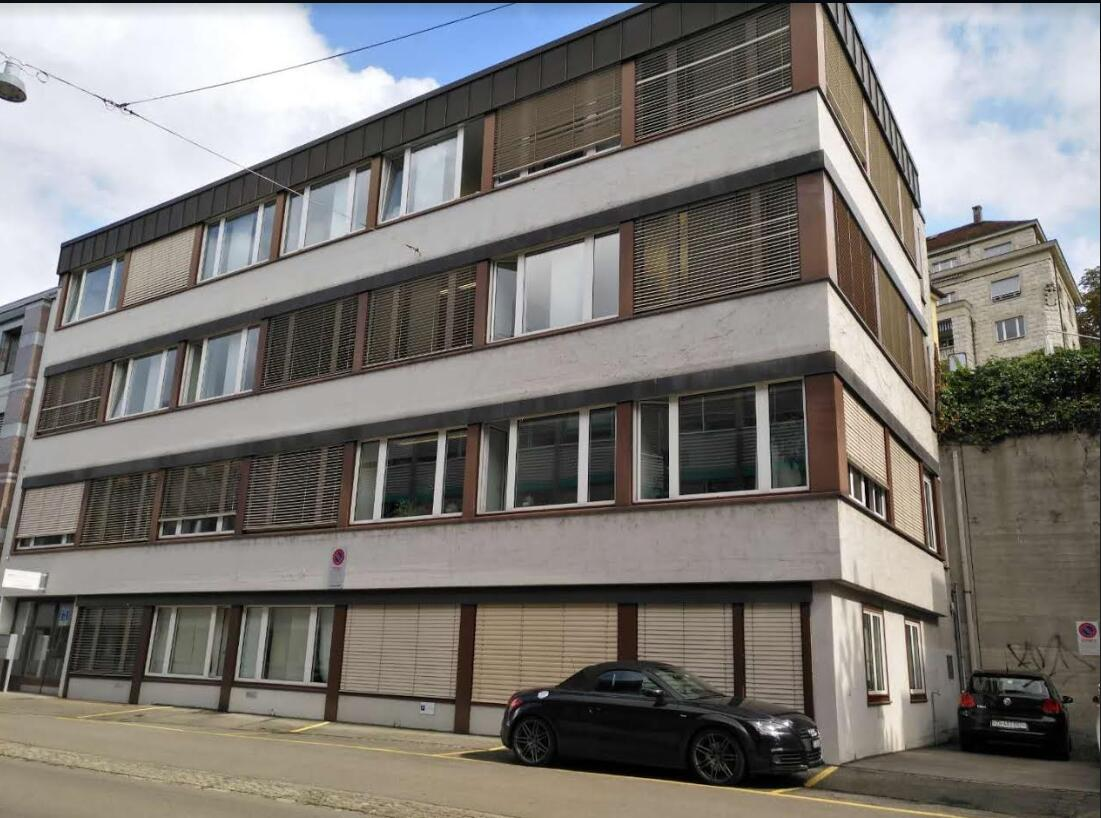
\includegraphics[scale=0.5]{Sumatra_photo.jpg}
		\caption{Sumatrastrasse 10 Office Building}
		\label{fig:Sumatra_photo}
		\end{figure}
		 
		
		According to the given information, the office building is constructed in 1951 and is located at Sumatrastrasse 10, 8006 Zurich, Switzerland. The building has 4 floors and a basement. The building  is facing west, and the window-to-wall ratio is 59\% on its west and south facade. The east facade of its ground floor and first floor is submerged into ground and there are heavy cover of plants on the upper floors with only a few necessary windows. There is also an underground floor used as warehouse and it's not included in any building model in this thesis.\\

		Figure \ref{fig:sumatra_og2} and \ref{fig:sumatra_og3} below are the floor plans of the building.
		The floor layout of ground floor, first floor and second floor are thought to be identical, and the third would have some small differences. For each floor, there is a toilet, a small office and 2 middle offices and a staircase. There is also a big office in each floor at the south side at ground floor, first floor and second floor. At the third floor, part of the big office and the corridor become a meeting room and a small pastry area as shown in the figures below. The detail building envelope material and modelling parameters are at chapter \textit{Methodology}.
		
		\begin{figure}[H]
		  \centering
		  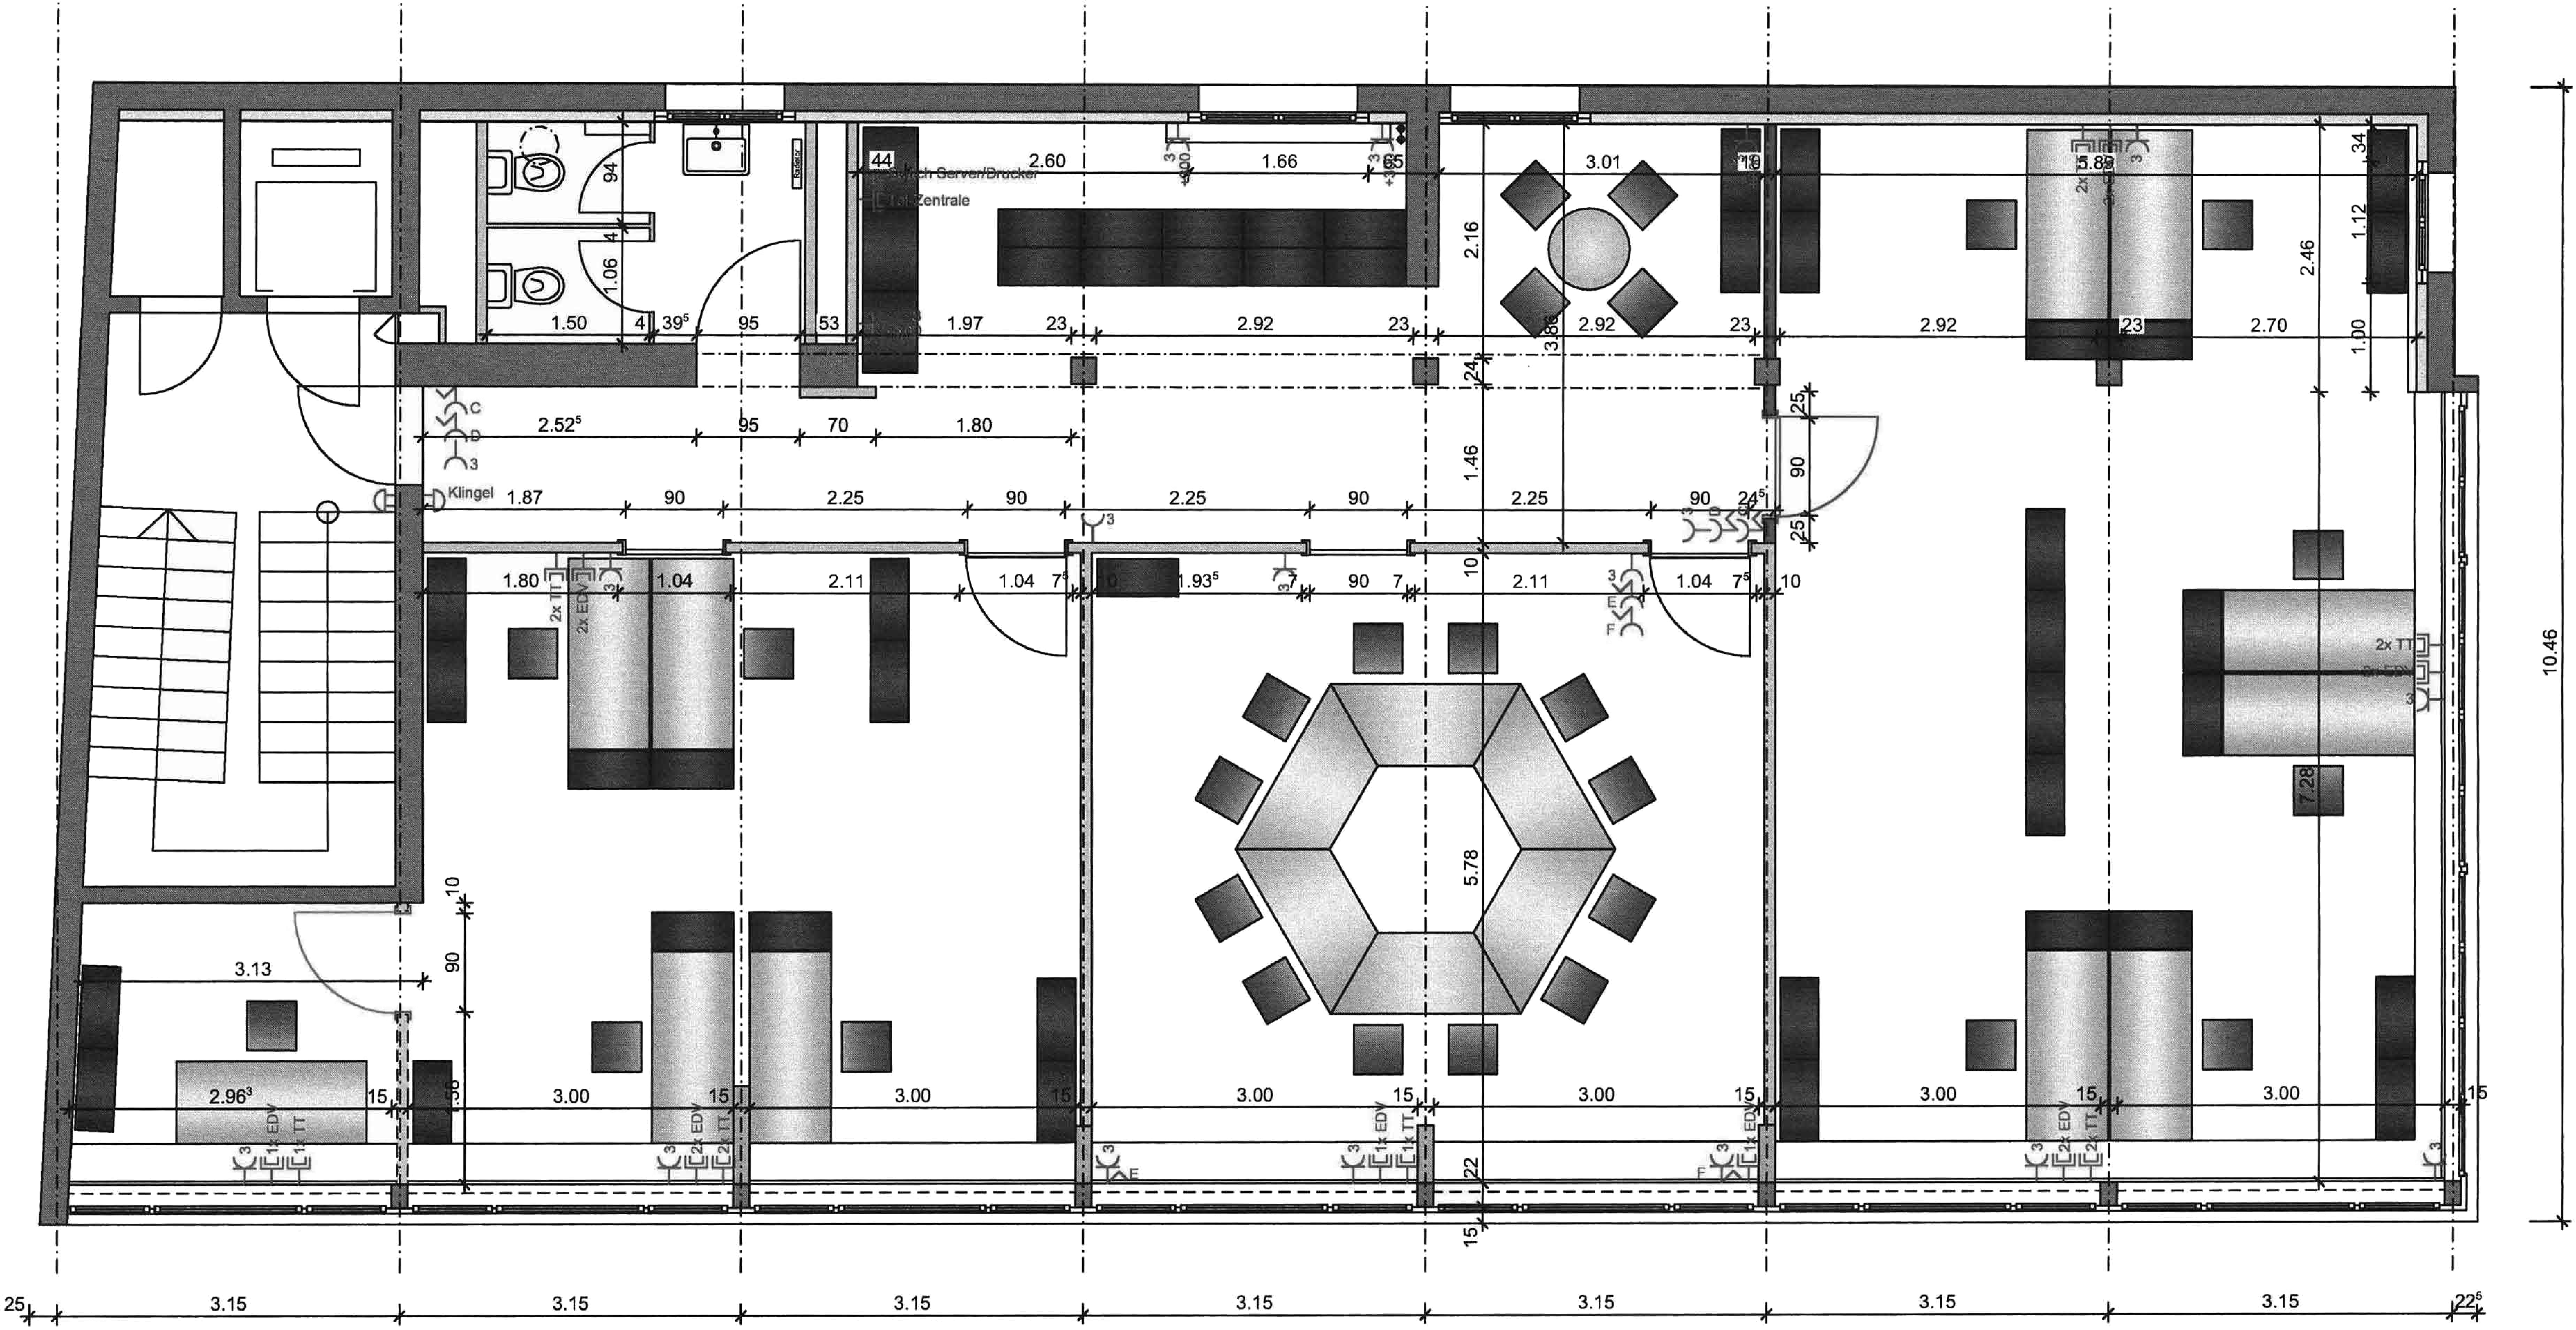
\includegraphics[scale=0.13]{Sumatra_OG2_Plan.pdf}
		  \caption{Floor plan of office building (Sumatra) ground floor to 2$^{nd}$ floor}
		  \label{fig:sumatra_og2}
		 \end{figure}

		\begin{figure}[H]
		  \centering
		  \includegraphics[scale=0.13]{Sumatra_OG3_Plan.pdf}
		  \caption{Floor plan of office building (Sumatra) 3$^{rd}$ floor}
		  \label{fig:sumatra_og3}
		\end{figure}
	
	\newpage		
	\subsection{Residential Building Introduction}
		Figure \ref{fig:hongg_NE} and \ref{fig:hongg_SW} below show the photo of the residential building. The residential building is a part of a multi-family town house constructed in 1894. It is located at Honggerstrasse 23, 8037 Zurich, Switzerland. The building has 5 floors, the top floor is a loft and there is also an extra basement. There are 4 apartments in the building. The first apartment occupies the ground floor and the first floor, and the other 3 apartments each occupy one floor. Figure \ref{fig:hongg_eg_plan} and Figure \ref{fig:hongg_og1_plan} below are the floor plans of the residential building. The ground floor is connected with the first floor internally via a small staircase behide the kitchen. The black and red lines in Figure \ref{fig:hongg_eg_plan} show the ground floor layout and the yellow line indicates the layout of the upper floor. Similarily, Figure \ref{fig:hongg_og1_plan} shows the floor plans from first floor upward. The  red line indicates the layout of first floor and the yellow line shows the layout from second floor up. The detail building envelope material and modelling parameters are at chapter \textit{Methodology}.\\
		

		\begin{figure}[htbp]
		\centering
		\begin{minipage}[t]{0.48\textwidth}
		\centering
		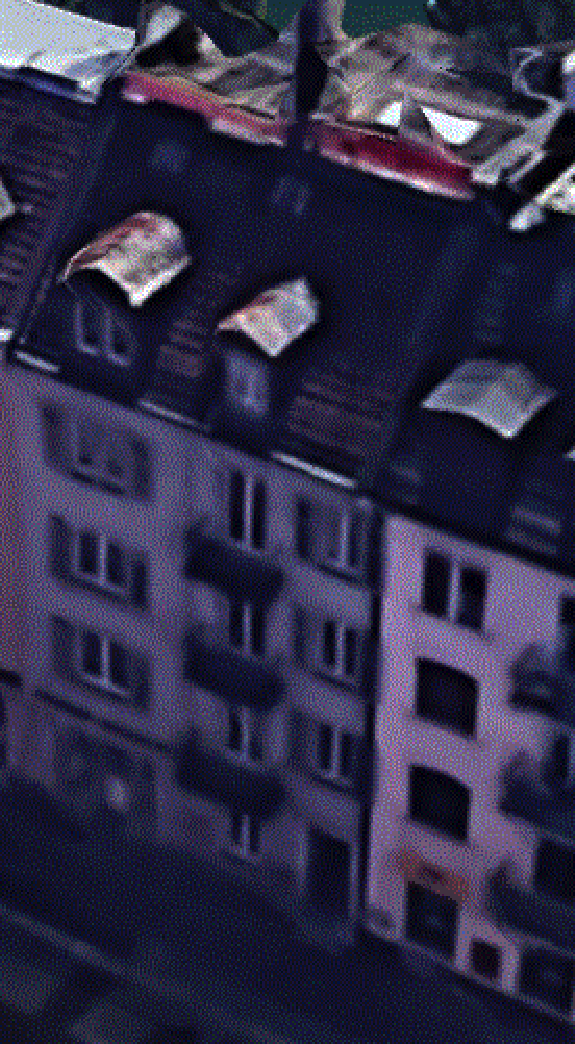
\includegraphics[width=5cm]{Hongg_photo1.pdf}
		\caption{Honggerstrasse 23, NE Side}
		\label{fig:hongg_NE}
		\end{minipage}
		\begin{minipage}[t]{0.48\textwidth}
		\centering
		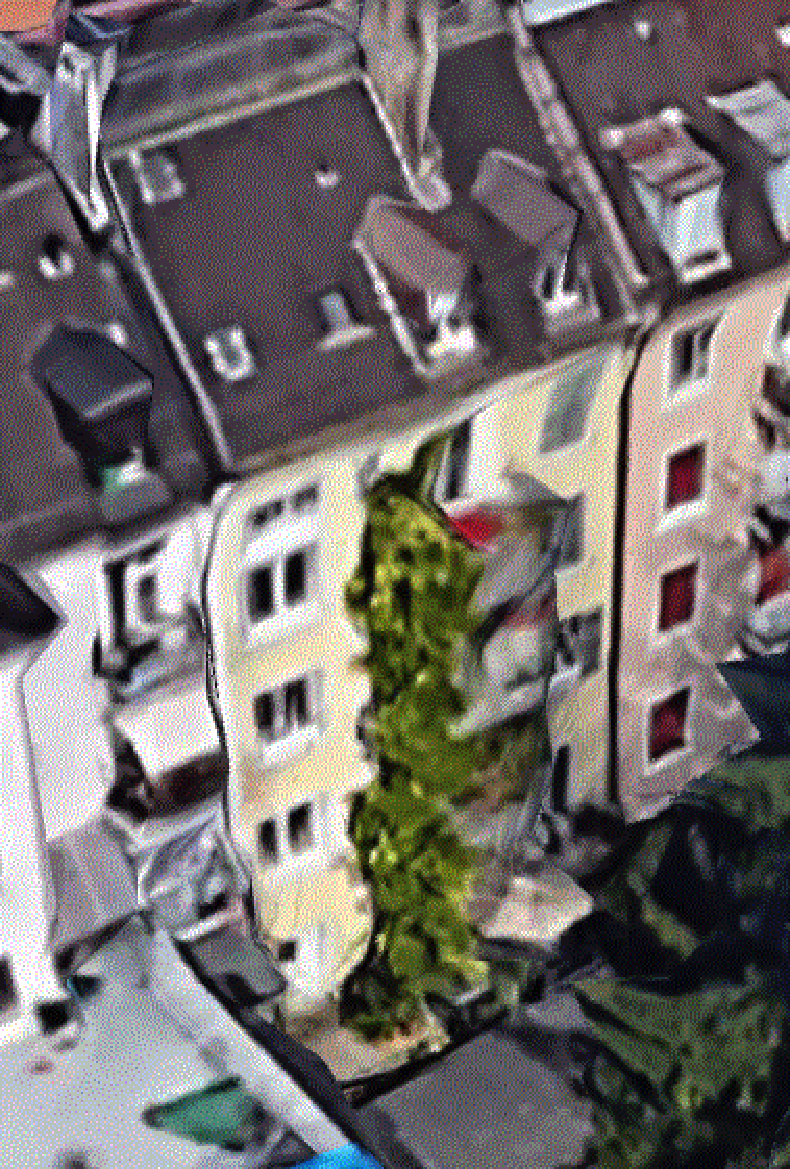
\includegraphics[width=6cm]{Hongg_photo0.pdf}
		\caption{Honggerstrasse 23, SW side}
		\label{fig:hongg_SW}
		\end{minipage}
		\end{figure}

		\begin{figure}[H]
		\centering
		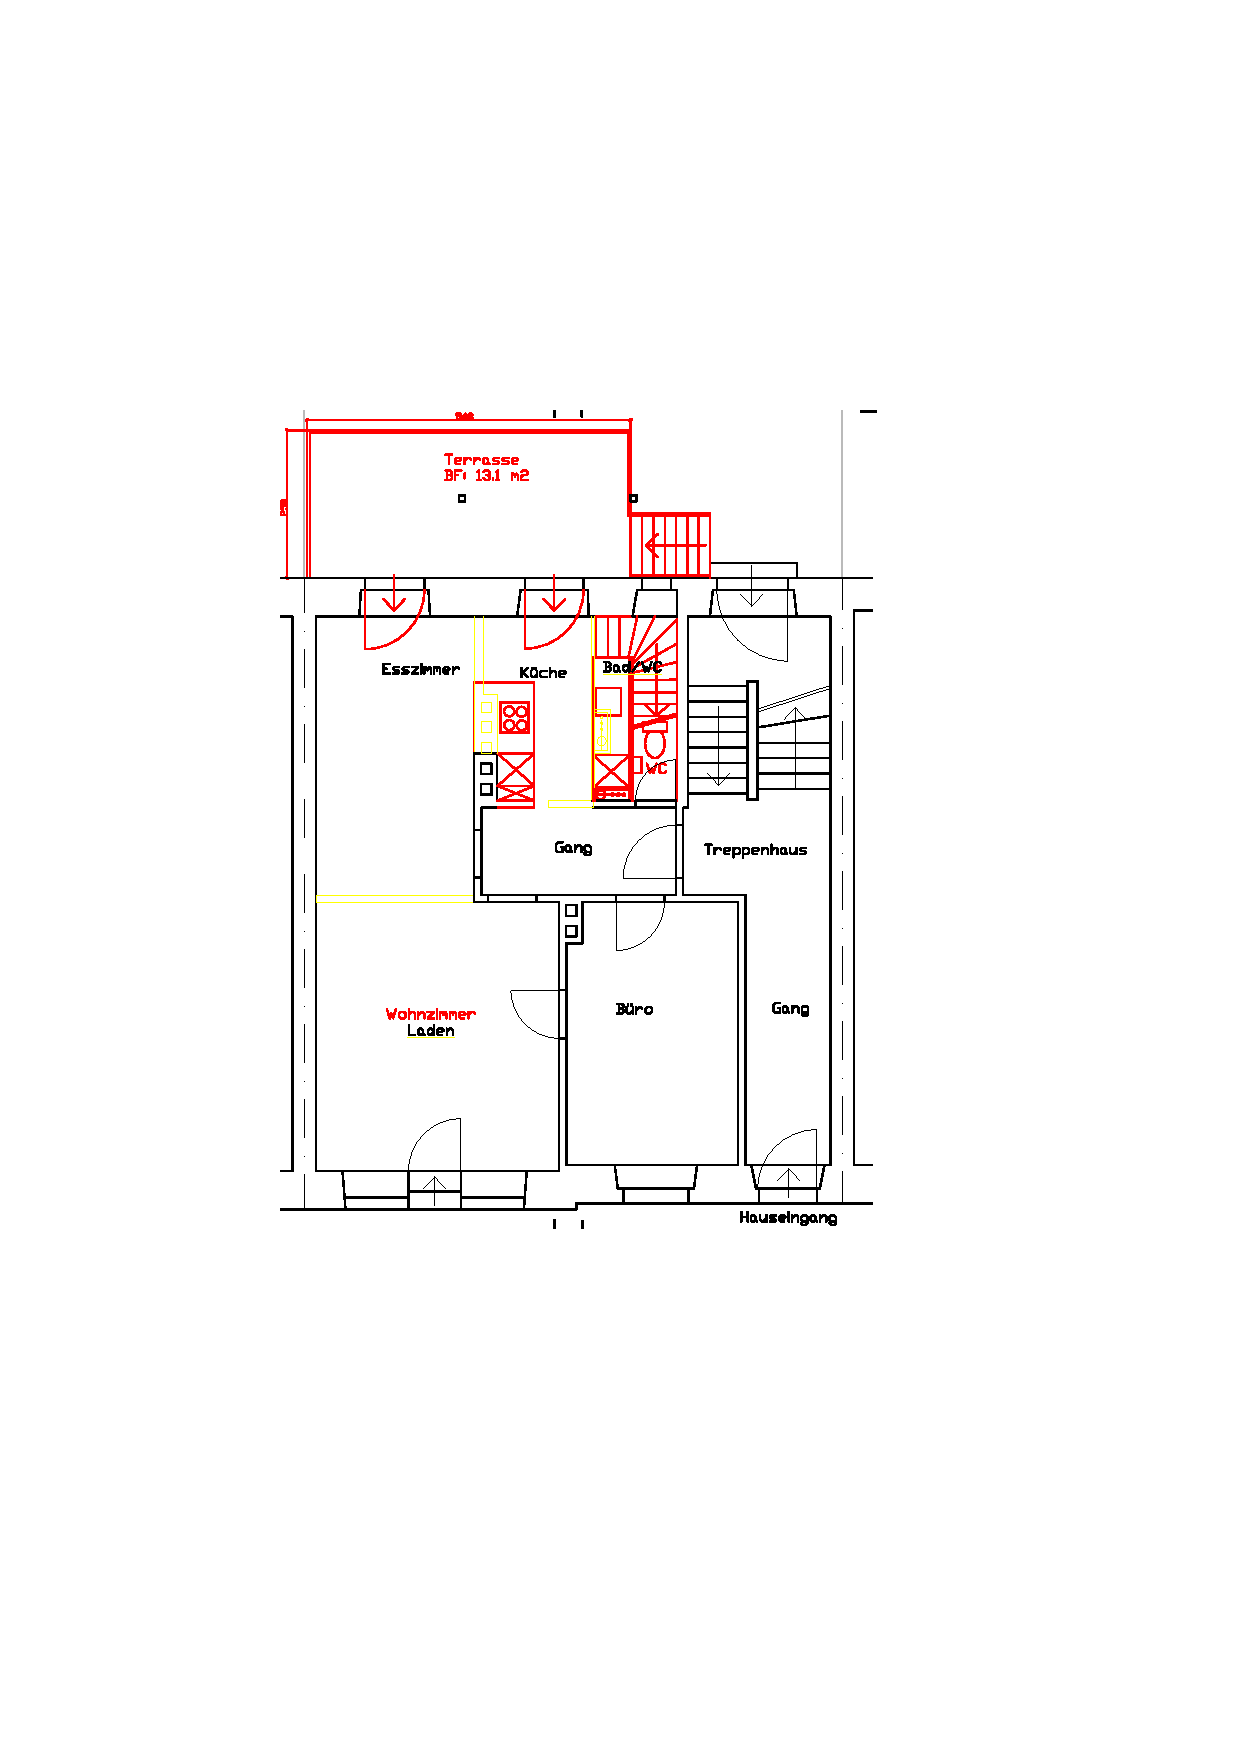
\includegraphics[scale=1.4]{Hongg_EG_Plan.pdf}
		\caption{Floor plan of residential building (Hongger) ground - 1$^{st}$ floor}
		\label{fig:hongg_eg_plan}
		\end{figure}
		
		\begin{figure}[H]
		\centering
		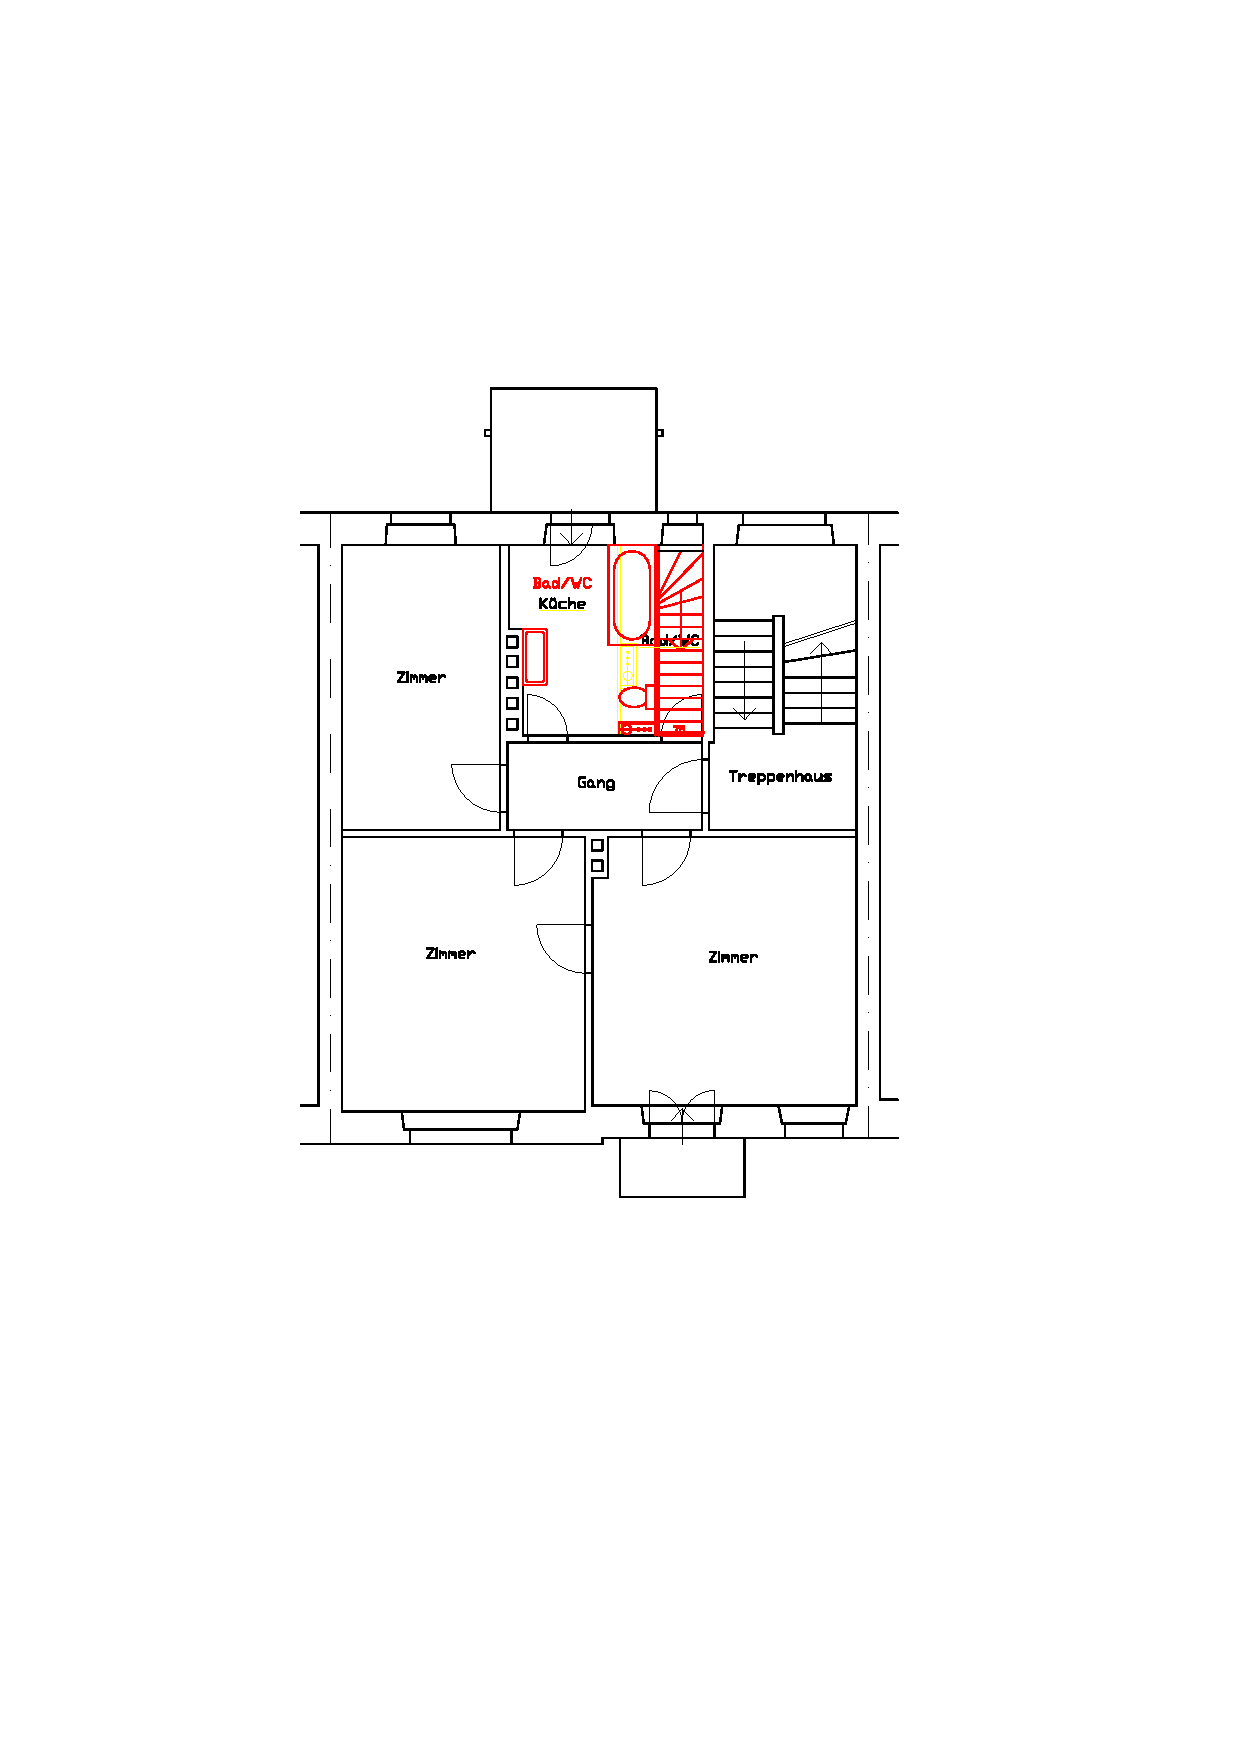
\includegraphics[scale=1.6]{Hongg_1OG_Plan.pdf}
		\caption{Floor plan of residential building (Hongger) 1$^{st} - 4^{th}$ floor}
		\label{fig:hongg_og1_plan}
		\end{figure}


	\subsection{Building Model Construction}
		\textit{DesignBuilder} is used to model the building envelopes of both buildings. It is compatible with EnergyPlus and provides advanced tools to model building geometry and building system.

		A brief introduction of DesignBuilder, also describe the scope of work (Building envelope, create a formated file for EnergyPlus engine, also provide accurate geometry data for SIA calculation)
		
		\subsubsection{Building Geometry}
			The actual geometry of the building is not specifically given in the previous report. However, a detailed floor plan and some geometries are given in pdf format as shown above in Figure \ref{fig:sumatra_og2}, and \ref{fig:sumatra_og3}, \ref{fig:hongg_eg_plan}, \ref{fig:hongg_og1_plan}. Therefore, in order to obtain an accurate building geometry, the pdf floor plan is firstly scaled to fit its nominated geometry, then a drawing file with correct scales are made according to the given pdf floor plans. After the drawing files are completed, they can be imported to DesignBuilder as a construction basis as shown in Figure \ref{fig:SumatraDxf} and \ref{fig:HonggerDxf} below.

			\begin{figure}[H]
			\centering
			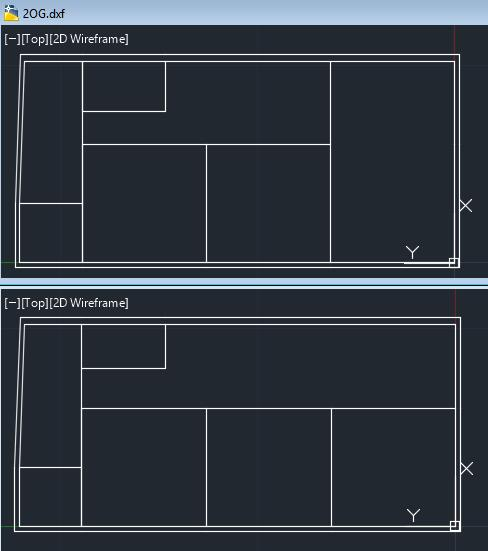
\includegraphics[scale=0.7]{Sumatra_dxf.jpg}
			\caption{dxf drawing files for office building}
			\label{fig:SumatraDxf}
			\end{figure}
			
			\begin{figure}[H]
			\centering
			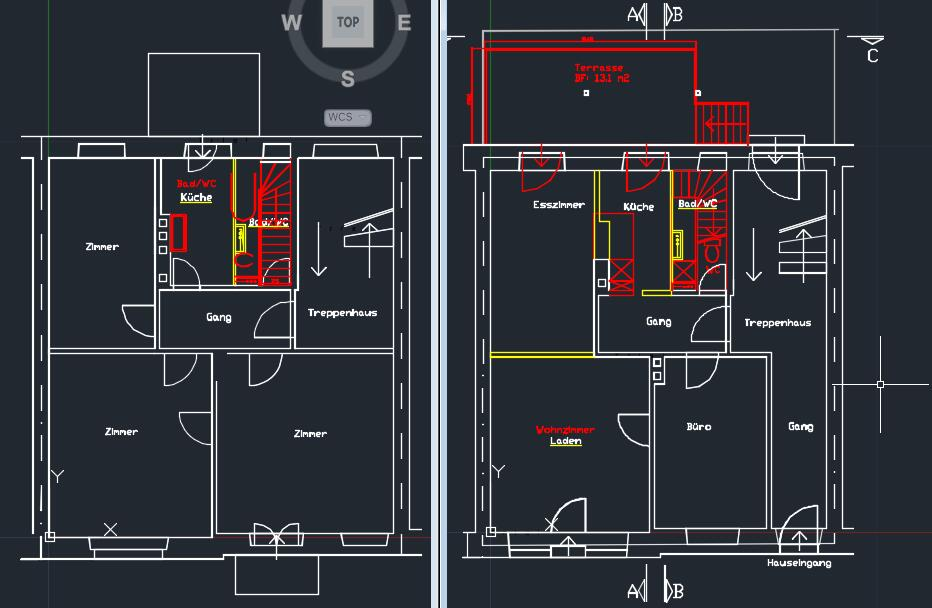
\includegraphics[scale=0.65]{Hongger_dxf.jpg}
			\caption{dxf drawing files for residential building}
			\label{fig:HonggerDxf}
			\end{figure}
			

			After the outline of buildings are constructed, windows and doors are defined. The window and door geometries of the office building and the residential building are shown at the table \ref{table:HonggerWindowLayout} and table \ref{table:SumatraWindowLayout} below. The detailed window code information can be found in Table \ref{tab:SumatraWindow}. \\

				%\newpage
				\begin{table}[H]
				\centering
				\caption{Window Layout of Residential Building}
				\begin{tabular}{  c | c | c | c  }
					\hline
					\multicolumn{4}{c}{Ground Floor} \\ 
					\hline
					Orientation & Location & Window Code & \# of window \\ \hline
					\multirow{4}{*}{SW} & Terrasse & 2a & 2 \\ 
					 & WC & 3a & 1 \\ 
					 & Staircase & 1a & 1 \\ 
					 & Front Door & TH & 1 \\ \hline
					\multirow{3}{*}{NE} & Laden & 1a & 1 \\ 
					 & Office & 4a & 1 \\ 
					 & Door & TH 1a & 1 \\ \hline
					\multicolumn{4}{c}{1st Floor to 4th Floor}\\ \hline
					\multirow{4}{*}{SW} & Terrasse & 2a & 1 \\ 
					 & WC & 3a & 1 \\ 
					 & Office & 4a & 1 \\ 
					 & Corridor & TH 1a & 1 \\ \hline
					\multirow{2}{*}{NE} & Office & 4a & 2 \\ 
					 & Terrasse & 2a & 1 \\ 
					 \hline
				\end{tabular}
				\label{table:HonggerWindowLayout}
				\end{table}


				\begin{table}[H]
				\centering
				\caption{Window Layout of Office Building}
				\begin{tabular}{  c | c | c | c  }
					\hline
					\multicolumn{4}{c}{Ground Floor}\\
					\hline
					Orientation & Location & Code & Number \\ \hline
					\multirow{4}{*}{W} & Right Office & FE1 & 2 \\
					 & Conference room & FE1 & 2 \\
					 & Large office & FE1 & 2 \\
					 & Corridor & FE6 & 2 \\ \hline
					S & Large office & FE6 & 2 \\ \hline
					\multicolumn{4}{c}{1st Floor and 2nd Floor}\\\hline
					\multirow{4}{*}{W} & Right Office & FE1 & 2 \\ 
					 & Conference room & FE1 & 2 \\ 
					 & Large office & FE1 & 2 \\ 
					 & small office & FE1 & 1 \\ \hline
					S & Large office & FE1 & 1 \\ \hline
					\multicolumn{4}{c}{3rd Floor}\\ \hline
					\multirow{4}{*}{W} & Right Office & FE1 & 2 \\ 
					 & Middle office & FE1 & 2 \\ 
					 & Corner office & FE1 & 2 \\ 
					 & small office & FE1 & 1 \\ \hline
					\multirow{3}{*}{S} & Corner office & FE1 & 2 \\ 
					 & Kitchen and Corridor & FE4 & 1 \\ 
					 & Kitchen and Corridor & FE5 & 1 \\ \hline
					\multirow{2}{*}{E} & Kitchen and Corridor & FE7 & 1 \\ 
					 & Staircase & FE3 & 1 \\ \hline
				\end{tabular}
				\label{table:SumatraWindowLayout}
				\end{table}


			
				\begin{table}[H]
				\centering
				\caption{Office building window specification}
			    \begin{tabular}{ccccc}
			    	\toprule
				    \multicolumn{1}{p{3em}}{Code} & \multicolumn{1}{p{3.785em}}{U-Value W/m2K} & \multicolumn{1}{p{4.215em}}{\#} & \multicolumn{1}{p{4.215em}}{unit area} & \multicolumn{1}{p{4em}}{Total Area m$^2$} \\
				    \midrule
				    \multicolumn{1}{c}{FE1} & 2.001 & 33   & 6    & 198 \\
				    \midrule
				    \multicolumn{1}{c}{FE2} & 2.500 & 1    & 8.125 & 8.13 \\
				    \midrule
				    \multicolumn{1}{c}{FE3} & 2.500 & 1    & 2.7  & 2.7 \\
				    \midrule
				    FE4  & 2.048 & 3    & 3.5  & 10.5 \\
				    \midrule
				    FE5  & 2.072 & 3    & 2.598 & 7.79 \\
				    \midrule
				    FE6  & 2.028 & 2    & 2.25 & 4.5 \\
				    \midrule
				    FE7  & 2.042 & 2    & 2.88 & 5.76 \\
				    \midrule
				    FE8  & 1.907 & 3    & 0.975 & 2.93 \\
				    \bottomrule
			    \end{tabular}%
				\label{tab:SumatraWindow}%
				\end{table}%

				% Table generated by Excel2LaTeX from sheet 'HonggerWindows'
				\begin{table}[H]
				\centering
				\caption{Residential building window specification}
				    \begin{tabular}{ccccc}
				    \toprule
				    \multicolumn{1}{p{4.215em}}{Code} & \multicolumn{1}{p{5.145em}}{U-Value W/m2K} & \multicolumn{1}{p{5.145em}}{number of windows} & \multicolumn{1}{p{4.43em}}{unit area} & \multicolumn{1}{p{5.145em}}{Total Area} \\
				    \midrule
				    FE-EG-1a & 2.379 & 1    & 6.9  & 9.9 \\
				    \midrule
				    FE-EG-2a & 2.388 & 10   & 2.6  & 26 \\
				    \midrule
				    FE-EG-3a & 2.19 & 5    & 0.6  & 3 \\
				    \midrule
				    FE-EG-4a & 2.285 & 13   & 1.6  & 20.8 \\
				    \midrule
				    FE-TH-1a & 2.33 & 1    & 2.88 & 3.7 \\
				    \midrule
				    Tur-TH & 3.5  & 1    & 2.5  & 2.5 \\
				    \bottomrule
				    \end{tabular}%
				\label{tab:HonggWindow}%
				\end{table}%


			
		

		\subsubsection{Building Envelope Material}
			After the building geometry is construct, the building wall and window elements are then assigned a set of thermal properties based on measurememt.
			Both buildings are uninsulated reinforced concrete structure buildings with thin outer and inner plaster layers. The detailed building wall material of both buildings as well as their thermodynamic properties are measured from the actural building and shown in Table \ref{tab:SumatraWallMaterial} and Table \ref{tab:HonggerWallMat}. The window properties and geometries of both buildings can be found in \ref{tab:SumatraWindow} and \ref{tab:HonggWindow}. Also note that the office building has PV panels on the roof but they are not included in either building geometry or building envelop. After the building material are assigned to all part of the buildings, static calculation and dynamic calculation can be performed.\\

			
			\newpage
			\begin{table}[h!]
			  \centering
			\caption{Wall material list of office building}
			    \begin{tabular}{rrrrrrr}
			    \toprule
			         & \multicolumn{1}{p{4em}}{Thickness \newline{}m} & \multicolumn{1}{p{3.145em}}{Density \newline{}kg/m3} & \multicolumn{1}{p{3.285em}}{Lambda \newline{}W/MK} & \multicolumn{1}{p{3.57em}}{Heat Capacity\newline{} KJ/Kg.K} & \multicolumn{1}{p{2.93em}}{R Value \newline{}m2K/W} & \multicolumn{1}{p{3.145em}}{U Value \newline{}W/m2K} \\
			    \midrule
			    \multicolumn{7}{p{26.86em}}{EG East Wall} \\
			    \multicolumn{1}{l}{Outside convection coefficient} &      &      &      &      &      &  \\
			    \multicolumn{1}{p{6.785em}}{Outer Layer} & 0.36 & 2400 & 2.5  & 1    & 0.144 &  \\
			    \multicolumn{1}{p{6.785em}}{Inner Layer} & 0.01 & 1400 & 0.7  & 1    & 0.014 &  \\
			    \multicolumn{3}{p{13.93em}}{Inside convection coefficientr} &      &      & 0.13 & 7.7 \\
			         &      &      &      &      & 0.288 & 3.4703 \\
			    \midrule
			    \multicolumn{7}{p{26.86em}}{West and Other Wall} \\
			    \multicolumn{4}{p{17.215em}}{Outside convection Coefficient} &      & 0.04 & 25 \\
			    \multicolumn{1}{p{6.785em}}{Outside Layer} & 0.02 & 1400 & 0.7  & 1    & 0.029 & 35 \\
			    \multicolumn{1}{p{6.785em}}{Layer2} & 0.05 & 1100 & 0.44 & 0.94 & 0.114 & 8.8 \\
			    \multicolumn{1}{p{6.785em}}{Middle Layer} & 0.02 & 120  & 0.056 & 1.56 & 0.357 & 2.8 \\
			    \multicolumn{1}{p{6.785em}}{Inside Layer} & 0.15 & 2400 & 2.5  & 1    & 0.06 & 16.667 \\
			    \multicolumn{4}{p{17.215em}}{Inside Convection Coefficient} &      & 0.13 & 7.7 \\
			         &      &      &      &      & 0.729 & 1.3713 \\
			    \midrule
			    \multicolumn{7}{p{26.86em}}{East Wall (Thick)} \\
			    \multicolumn{3}{p{13.93em}}{Outside convection Coefficient} &      &      & 0.04 & 25 \\
			    \multicolumn{1}{p{6.785em}}{Outside Layer} & 0.02 & 1800 & 0.87 & 1    & 0.023 & 43.5 \\
			    \multicolumn{1}{p{6.785em}}{Middle Layer} & 0.36 & 1100 & 0.44 & 0.94 & 0.818 & 1.2222 \\
			    \multicolumn{1}{p{6.785em}}{Inside Layer} & 0.02 & 1400 & 0.7  & 1    & 0.029 & 35 \\
			    \multicolumn{3}{p{13.93em}}{Inside Convection Coefficient} &      &      & 0.13 & 7.7 \\
			         &      &      &      &      & 1.04 & 0.9619 \\
			    \midrule
			    \multicolumn{7}{p{26.86em}}{Ceiling} \\
			    \multicolumn{3}{p{13.93em}}{Outside convection coefficient} &      &      & 0.04 & 25 \\
			    \multicolumn{1}{p{6.785em}}{Layer 1} & 0.04 & 120  & 0.056 & 1.56 & 0.714 &  \\
			    \multicolumn{1}{p{6.785em}}{Layer 2} & 0.0042 & 1100 & 0.23 & 1    & 0.15 &  \\
			    \multicolumn{1}{p{6.785em}}{Layer 3} & 0.0035 & 1100 & 0.23 & 1    & 0.015 &  \\
			    \multicolumn{1}{p{6.785em}}{Layer 4} & 0.001 & 980  & 0.5  & 1.8  & 0.002 &  \\
			    \multicolumn{1}{p{6.785em}}{Layer 5} & 0.22 & 2400 & 2.5  & 1    & 0.088 &  \\
			    \multicolumn{3}{p{13.93em}}{Inside convection coefficientr} &      &      & 0.13 & 7.7 \\
			         &      &      &      &      & 1.139 & 0.8777 \\
			    \midrule
			    \multicolumn{7}{p{26.86em}}{Ground} \\
			    \multicolumn{3}{p{13.93em}}{Outside convection coefficient} &      &      & 0.13 & 7.7 \\
			    \multicolumn{1}{p{6.785em}}{Layer 1} & 0.01 & 120  & 0.056 & 1.56 & 0.179 &  \\
			    \multicolumn{1}{p{6.785em}}{Layer 2} & 0.22 & 2400 & 2.5  & 1    & 0.088 &  \\
			    \multicolumn{3}{p{13.93em}}{Inside convection coefficientr} &      &      & 0.13 & 7.7 \\
			         &      &      &      &      & 0.526 & 1.9 \\
			    \bottomrule
			    \end{tabular}%
			  \label{tab:SumatraWallMaterial}%
			\end{table}%

			\newpage
			\begin{table}[h!]
			  \centering
			\caption{Residential building wall material}
			    \begin{tabular}{rrrrrrr}
			    \toprule
			         & \multicolumn{1}{p{3.93em}}{Thickness m} & \multicolumn{1}{p{3.07em}}{Density kg/m3} & \multicolumn{1}{p{3.145em}}{Lambda W/MK} & \multicolumn{1}{p{3.57em}}{Heat Capacity KJ/Kg.K} & \multicolumn{1}{p{3.355em}}{R Value m2K/W} & \multicolumn{1}{p{3.355em}}{U Value W/m2K} \\
			    \midrule
			    \multicolumn{7}{c}{External Wall} \\
			    \midrule
			    \multicolumn{1}{l}{Outside convection Coefficient} &      &      &      &      & 0.04 & 25 \\
			    \multicolumn{1}{l}{Outside Layer} & 0.04 & 1800 & 0.87 & 1    & 0.046 & 21.75 \\
			    \multicolumn{1}{l}{Middle Layer} & 0.6  & 1800 & 0.8  & 0.94 & 0.75 & 1.3333 \\
			    \multicolumn{1}{l}{Inside Layer} & 0.02 & 1400 & 0.7  & 1    & 0.0286 & 35 \\
			    \multicolumn{1}{l}{Inside Convection Coefficient} &      &      &      &      & 0.1299 & 7.7 \\
			         &      &      &      &      & 0.9944 & 1.0056 \\
			    \midrule
			    \multicolumn{7}{c}{Ground} \\
			    \midrule
			    \multicolumn{1}{l}{Outside convection coefficient} &      &      &      &      & 0.1299 & 7.7 \\
			    \multicolumn{1}{l}{Layer 1} & 0.02 & 900  & 0.25 & 1    & 0.08 &  \\
			    \multicolumn{1}{l}{Layer 2} & 0.1  &      &      &      & 0.15 &  \\
			    \multicolumn{1}{l}{Layer 3} & 0.03 & 1500 & 1.5  & 2.1  & 0.02 &  \\
			    \multicolumn{1}{l}{Layer 4} & 0.03 & 500  & 0.13 & 1.6  & 0.2308 &  \\
			    \multicolumn{1}{l}{Inside convection coefficientr} &      &      &      &      & 0.1299 & 7.7 \\
			         &      &      &      &      & 0.7405 & 1.3504 \\
			    \midrule
			    \multicolumn{7}{c}{Ceiling} \\
			    \midrule
			    \multicolumn{1}{l}{Outside convection coefficient} &      &      &      &      & 0.1299 & 7.7 \\
			    \multicolumn{1}{l}{Layer 1} & 0.02 & 1400 & 0.7  & 1    & 0.0286 &  \\
			    \multicolumn{1}{l}{Layer 2} & 0.2  & 2300 & 2.3  & 1    & 0.087 &  \\
			    \multicolumn{1}{l}{Layer 3} & 0.02 & 1500 & 1.5  & 2.1  & 0.0133 &  \\
			    \multicolumn{1}{l}{Layer 4} & 0.03 & 500  & 0.13 & 1.6  & 0.2308 &  \\
			    \multicolumn{1}{l}{Inside convection coefficientr} &      &      &      &      & 0.1299 & 7.7 \\
			         &      &      &      &      & 0.6194 & 1.6145 \\
			    \bottomrule
			    \end{tabular}%
			  \label{tab:HonggerWallMat}%
			\end{table}%

		Figure \ref{fig:SumatraDB} and \ref{fig:HonggDB} below shows a completed office and residential building DesignBuilder model with geometry and material information.\\

			%\newpage
			\begin{figure}[H]
			\centering
			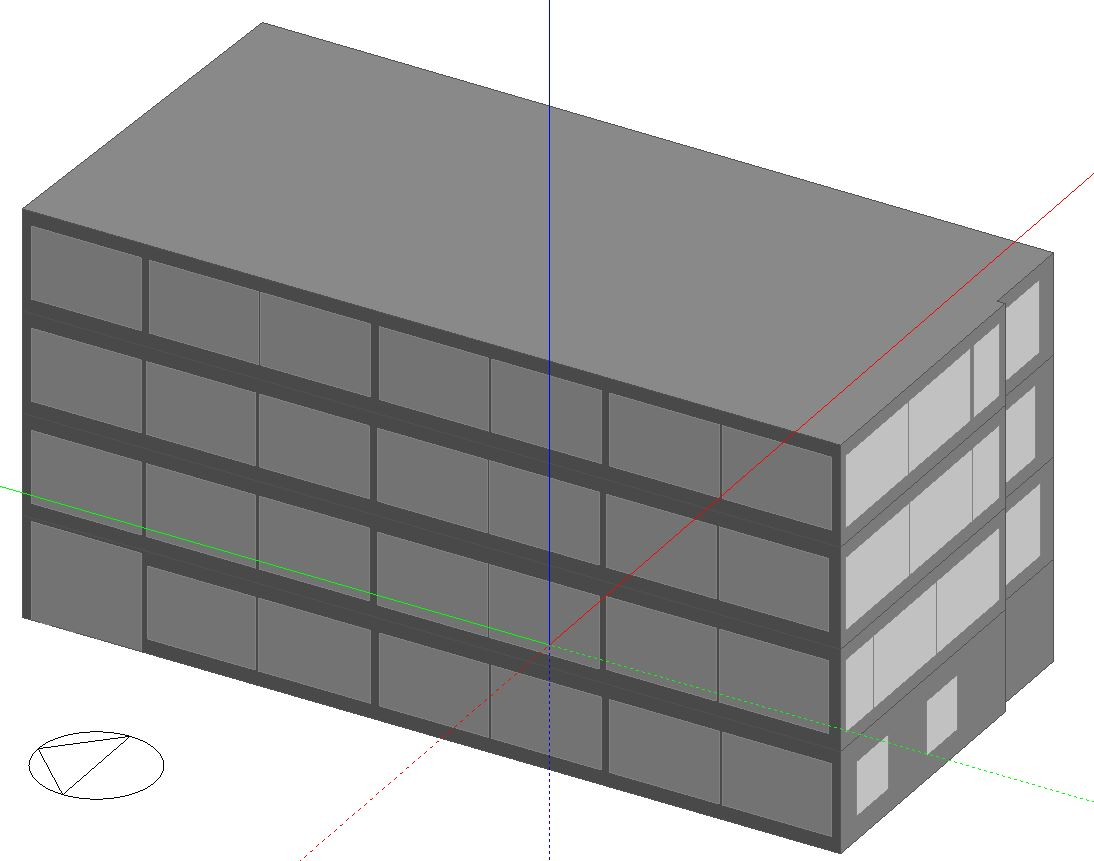
\includegraphics[scale=0.45]{SumatraDesignBuilderModel.JPG}
			\caption{Office building DesignBuilder model}
			\label{fig:SumatraDB}
			\end{figure}

			\begin{figure}[H]
			\centering
			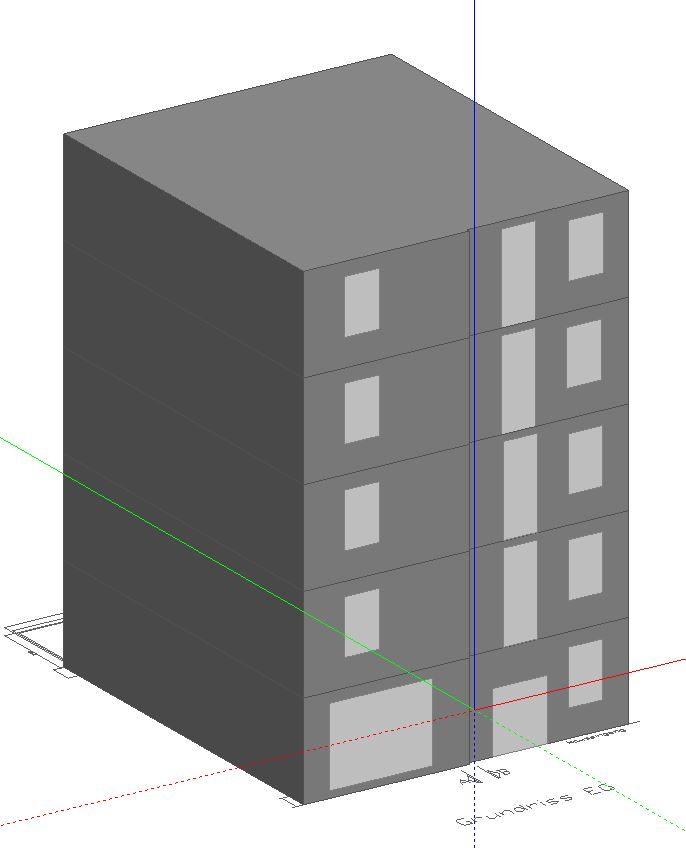
\includegraphics[scale=0.45]{HonggDesignBuilderModel.JPG}
			\caption{Residential building DesignBuilder model}
			\label{fig:HonggDB}
			\end{figure}

			\subsection{SIA Documentations}
		Most of the building occupancy and activity assumption are from the standard values published by the Swiss society of engineers and architects (hereinafter: SIA Standard). The SIA standards range from energy consumption calculation formulars to the supporting informations about a perticular building type or a room type. It also include a reference standard weather data set for most of the cities in Switzerland. Here are the main SIA standards that are used or taken into account in this thesis.\\

		\textbf{SIA 380/1: Thermal energy in buildings}\\
			This SIA standard is published in 2009 replacing its predecessor SIA 380/1 (2007). It is often used with other standardized calculation parameters when assessing the energy efficiency of existing buildings \cite{SIAPreviousreport}. It also serves as a forecasting tool to evaluate the refurbishment plans. However, the building usually consume less energy than what the calculation suggest, and this issue become more severe as the building envelope gets worse as hown in figure \ref{fig:SIA380PG} below. When using SIA 380/1 to calculate the entitlements for governmental energy certificates, standardized data is used, when using SIA 380/1 for energy consulting, design and optimizations, the best known data is used \cite{SIAPreviousreport}.\\




		\textbf{SIA 2028: SIA Weather Data}\\
			SIA also published a set of standard weather information for most cities in Switzerland. It separates Switzerland into several climate zones and each zone would have their specific climate patten and typical weather data for energy calculation. As SIA 380/1 use monthly average temperature and monthly heating degree days to calculate annual heating demand, this SIA standard weather data is used in this thesis as a reference guide.\\

			The weather data set include monthly and annual average temperature, monthly and annual heating degree days, monthly and annual solar radiation in north, south, east, west and horizontal surfaces. In addition, SIA also published another set of standard hourly data on its partner website \textit{www.energytool.ch} for purchase.\\

		\textbf{SIA 2024: SIA Occupancy and schedule}\\
			Apart from the standard calculation of SIA 380/1 which use monthly and annual unit area standard values for a specific building type, SIA also developed a dynamic building energy analysis approach which use hourly unit area data for a specific room or zone type. SIA 2024 is the unification of assumptions about occupancy and equipment or appliance usage level for specific zone types such as corridor, bedroom, living room and toilet.\\

			The assumptions listed in SIA 2024 include room heating and/or cooling setpoint, maximum supply wind speed, typical room area, window-to-wall ratio, window g-values, room occupancy level and activity level, internal gain level, electricity usage level and activities, minimum and typical amount of outdoor air and ventilation level, lighting and domestic hot water demand etc.\\

			These assumptions are used in calculations and verifications according to energy and building service standard. For occupancy and appliance level assumptions, it gives not only a specific value but also a resonable range which enable a stochastic building energy consumption analysis. SIA 2024 has provide assumptions for 46 different zone types, which cover a majority of building types \cite{SIA2024Shop}.




	


	\newpage

		\subsection{Weather Data Selection}
			A number of data files or weather data are used during this research. These weather files and data include a typical SIA standard monthly weather and hourly weather; a typical hourly weather file which contains an average or typical weather information from the recent 10 to 15 years; a created data file based on weather station measurement in 2015, and a created heat island weather file. These weather data can be grouped into two categories according to their functions.

			\subsubsection{Weather Data For Static Calculation}
			\textbf{SIA 381/2 Weather Data}\\
				SIA has published a standard weather data \textit{SIA 381/2 Klimadaten zi Emfehlung SIA 380/1} (Recommended climate data for SOA 380/1) in 1988. It separate Switzerland into a number of climate zones. It also contain monthly weather data set for most main cities in Switzerland. The useful information from this weather dataset are monthly air temperature, monthly heating days, monthly heating degree days and monthly solar radiation on different orientation surfaces.\\


				\begin{table}[H]
				  \centering
				  \small
				\caption{SIA 381/2 Weather Data}
				    \begin{tabular}{|p{5.355em}|c|c|c|c|c|c|c|c|c|c|c|c|c|}
				    \toprule
				    \multicolumn{14}{|c|}{SIA 381/2 Weather Data} \\
				    \midrule
				    \textbf{Month} & \textbf{Jan} & \textbf{Feb} & \textbf{Mar} & \textbf{Apr} & \textbf{May} & \textbf{Jun} & \textbf{Jul} & \textbf{Aug} & \textbf{Sep} & \textbf{Oct} & \textbf{Nov} & \textbf{Dec} & \textbf{Sum} \\
				    \midrule
				    Average Temperature & 0.1  & 2.1  & 4.8  & 9    & 14   & 18   & 19   & 18   & 16   & 11   & 5.4  & 0.6  & 3260 \\
				    \midrule
				    HDD  & 615  & 501  & 467  & 255  & 110  & 23   & 7    & 6    & 35   & 207  & 433  & 601  & 1091 \\
				    \midrule
				    Solar Energy at N (MJ/m2) & 33   & 48   & 78   & 108  & 158  & 172  & 168  & 116  & 89   & 61   & 32   & 28   & 2248 \\
				    \midrule
				    Solar Energy at E (MJ/m2) & 57   & 96   & 170  & 243  & 299  & 320  & 330  & 284  & 212  & 127  & 61   & 49   & 3133 \\
				    \midrule
				    Solar Energy at S (MJ/m2) & 149  & 217  & 281  & 315  & 299  & 290  & 318  & 337  & 347  & 272  & 166  & 142  & 2303 \\
				    \midrule
				    Solar Energy at W (MJ/m2) & 67   & 110  & 170  & 248  & 294  & 308  & 330  & 284  & 227  & 138  & 70   & 57   & 4156 \\
				    \midrule
				    Horizontal Solar Energy & 94   & 166  & 299  & 450  & 565  & 616  & 648  & 526  & 385  & 227  & 104  & 76   & 1564 \\
				    \midrule
				    Solar Energy at NE & 43   & 68   & 115  & 162  & 217  & 235  & 235  & 182  & 137  & 88   & 44   & 37   & 2653 \\
				    \midrule
				    Solar Energy at SW & 100  & 154  & 219  & 279  & 296  & 299  & 324  & 309  & 281  & 194  & 108  & 90   & 2653 \\
				    \bottomrule
				    \end{tabular}%
				  \label{tab:WeatherSIA3812}%
				\end{table}%



			\textbf{2015 Weather Data}\\
				The 2015 Zurich weather data for static calculation is based on the information from the given 2015 .\textit{epw} weather file. The hourly data is firstly extracted from the weather file then calculate the monthly average. \textit{Rhino6} and \textit{Grasshopper} are also used to extract the hourly data as well as calculating the average monthly solar radiation on the nominal orientations (N, E, S, W, NE, SW, and Horizontal). The resultant monthly weather data is shown at Table \ref{tab:2015Monthly}. Table \ref{tab:StaticWeatherCompare} below indicate a comparison of two different weather data.
				
				\begin{table}[H]
				  \centering
				  \small
				\caption{2015 Zurich Monthly Data}
				    \begin{tabular}{|p{5.3em}|r|r|r|r|r|r|r|r|r|r|r|r|r|}
				    \toprule
				    \multicolumn{14}{|c|}{2015 Weather Data} \\
				    \midrule
				    \textbf{Month} & \multicolumn{1}{l|}{\textbf{Jan}} & \multicolumn{1}{l|}{\textbf{Feb}} & \multicolumn{1}{l|}{\textbf{Mar}} & \multicolumn{1}{l|}{\textbf{Apr}} & \multicolumn{1}{l|}{\textbf{May}} & \multicolumn{1}{l|}{\textbf{Jun}} & \multicolumn{1}{l|}{\textbf{Jul}} & \multicolumn{1}{l|}{\textbf{Aug}} & \multicolumn{1}{l|}{\textbf{Sep}} & \multicolumn{1}{l|}{\textbf{Oct}} & \multicolumn{1}{l|}{\textbf{Nov}} & \multicolumn{1}{l|}{\textbf{Dec}} & \multicolumn{1}{l|}{\textbf{Sum}} \\
				    \midrule
				    Average Temperature  & 3.7  & 1.5  & 8.2  & 12   & 16   & 20   & 25   & 23   & 15   & 11   & 9    & 5.1  &  \\
				    \midrule
				    Heating Degree Days & 498  & 519  & 344  & 149  & 31   & 0    & 0    & 0    & 18   & 225  & 268  & 462  & 2513.1 \\
				    \midrule
				    Solar Energy at N (MJ/m2) & 25   & 42   & 62   & 86   & 116  & 158  & 150  & 107  & 74   & 46   & 30   & 23   & 919.15 \\
				    \midrule
				    Solar Energy at E (MJ/m2) & 55   & 103  & 176  & 238  & 289  & 301  & 332  & 278  & 185  & 113  & 65   & 41   & 2176.1 \\
				    \midrule
				    Solar Energy at S (MJ/m2) & 183  & 213  & 304  & 298  & 244  & 237  & 245  & 284  & 279  & 238  & 146  & 116  & 2786.3 \\
				    \midrule
				    Solar Energy at W (MJ/m2) & 67   & 97   & 186  & 233  & 261  & 294  & 299  & 258  & 206  & 127  & 61   & 52   & 2140.7 \\
				    \midrule
				    Horizontal Solar Energy & 104  & 174  & 316  & 446  & 549  & 596  & 605  & 512  & 353  & 208  & 108  & 78   & 4049.9 \\
				    \midrule
				    Solar Energy at NE & 26   & 51   & 92   & 140  & 202  & 231  & 244  & 179  & 108  & 58   & 33   & 24   & 1388.6 \\
				    \midrule
				    Solar Energy at SW & 146  & 167  & 269  & 287  & 273  & 282  & 288  & 290  & 268  & 204  & 112  & 97   & 2683.8 \\
				    \bottomrule
				    \end{tabular}%
				  \label{tab:2015Monthly}%
				\end{table}%

				% Table generated by Excel2LaTeX from sheet 'Sheet2'
				\begin{table}[htbp]
				  \centering
				\caption{Weather Data Comparison}
				    \begin{tabular}{|c|c|c|c|}
				    \toprule
				         & \multicolumn{1}{c}{SIA Standard Weather} & 2015 Weather & Typical Zurich Weather\\
				    \midrule
				    Heating Day & 208  & 175 & 213\\
				    \midrule
				    Heating Degree Day & 3260 & 2513 & 3283\\
				    \midrule
				    Annual Average Temperature & 8.5  & 12.3 & 9.75\\
				    \bottomrule
				    \end{tabular}%
				  \label{tab:StaticWeatherCompare}%
				\end{table}%


			\subsubsection{Weather Data For Dynamic Calculation}
				An .\textit{epw} weather file is needed for dynamic calculation using \textit{EnergyPlus}. The weather file is either from a meteological organization or from modifying an existing weather file. It contains a large number of weather information such as dry-bulb temperature, wet-bulb temperature, relative humidity, wind speed, wind direction, hourly solar radiation, cloudiness etc.\\

			\textbf{Typical Year Weather File}\\
				A typical year Zurich weather file is given by EMPA research unit. It also become the basis for other custom-made weather files that are used in this thesis. The basic statistic information of the typical year weather file is shown at the 3$^{rd}$ column of Table \ref{tab:StaticWeatherCompare}. \\

			\textbf{2015 Weather File}\\
				The 2015 weather file is created from the typical Zurich weather file by replacing the dry bulb temperature, wet bulb temperature, relative humidity, wind speed, and wind direction by the actual hourly measured data in Zurich in 2015. The source of weather data is from \textit{Federal Office of Meteology and Climatology MeteoSwiss}. Considering the location of the two existing building, the weather station is chosen to be \textit{NABZUE}, which located at Zurich city as shown in Figure \ref{fig:NABZUE}.

				\begin{figure}[H]
				\centering
				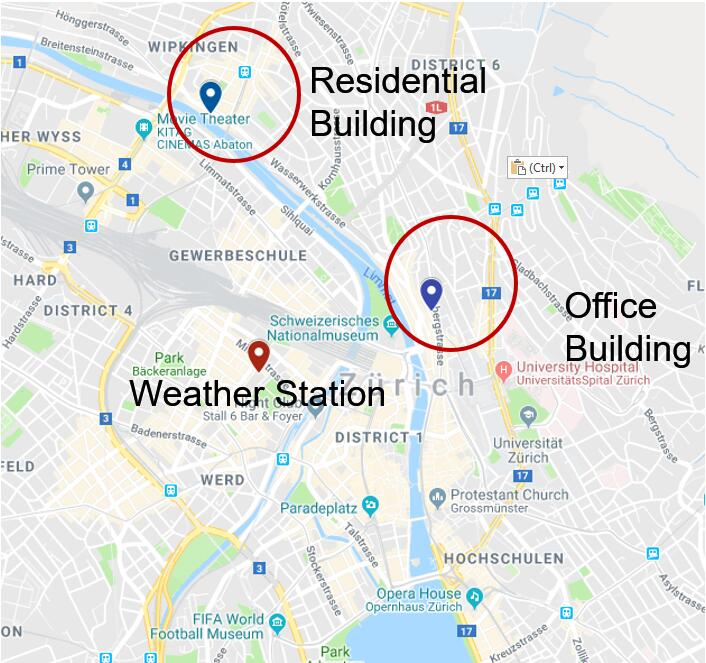
\includegraphics[scale=0.7]{WeatherStation.jpg}
				\caption{Weather Station Location}
				\label{fig:NABZUE}
				\end{figure}
				
				% Table generated by Excel2LaTeX from sheet 'Sheet2'
				\begin{table}[htbp]
				  \centering
				  \caption{Weather Data Information}
				    \begin{tabular}{|c|c|}
				    \toprule
				    \multicolumn{2}{|c|}{\textbf{2015 Weather Data Information}} \\
				    \midrule
				    Source & MeteoSwiss: IDAWEB \\
				    \midrule
				    Weather Station Code & NABZUE \\
				    \midrule
				    Station Coordinate & E 8o31’49” , N 47o22’39” \\
				    \midrule
				    Altitude & 409 m \\
				    \midrule
				    Year & 2015 \\
				    \bottomrule
				    \end{tabular}%
				  \label{tab:2015DataInformation}%
				\end{table}%



			\textbf{SIA382 Weather File}\\
				The full weather data is not fully accessible, and only the hourly temperature is obtained. However, the SIA 382 Weather File is only used to investigate the global warming effect in Zurich. The hourly stand weather temperature is used to replace the typical year weather temperature in the typical year weather file, while all other information remain the same as the 2015 weather data. The comparison between SIA 382 temperature and 2015 actual temperature \\ 

			\textbf{Heat Island Weather File}\\
				Similarly, heat island weather is created based on measured data in year 2015 and aimed to investigate the heat island effect of Zurich city. Firstly, the temperature difference between building site temperature and the weather station data is recorded and average temperature difference is taken hour by hour as shown in Figure \ref{fig:HeatIslandConst} below. Then, a simple rule is apply on the 2015 weather temperature for each hour and create a new heat island weather temperature as shown in Figure \ref{fig:HeatIslandRule}. Lastly, the new heat island temperature is imported to the .\textit{epw} weather file and become the \textit{heat island weather file}.


				\begin{figure}[H]
				\centering
				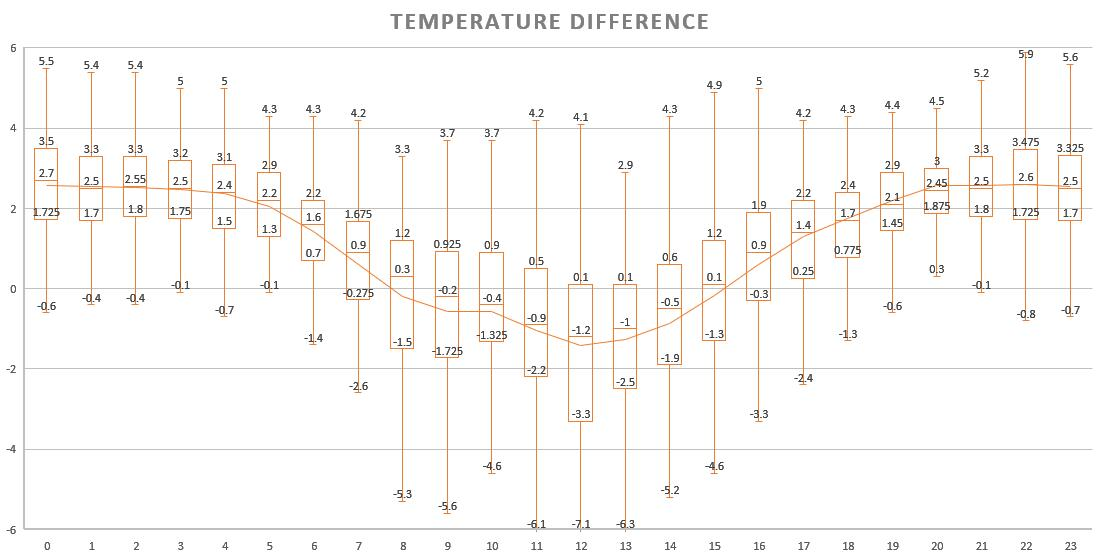
\includegraphics[scale=0.55]{HeatIsland_Construction.jpg}
				\caption{Temperature Difference}
				\label{fig:HeatIslandConst}
				\end{figure}
				
				\begin{figure}[H]
				\centering
				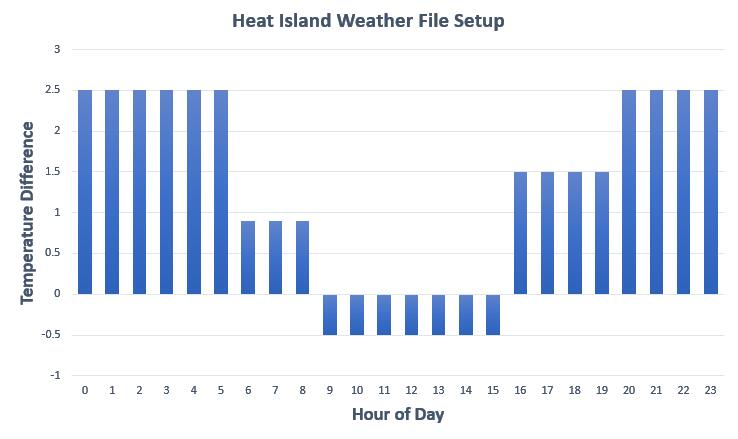
\includegraphics[scale=0.62]{HeatIslandConstruction.jpg}
				\caption{Heat Island Temperature Modification Rule}
				\label{fig:HeatIslandRule}
				\end{figure}
				



	\subsection{Static Calculation}
		To investigate the cause of huge deviation between previous static calculation and measurement heating demand, a new static calculation is conducted with more accurate geometry and weather information. As static calculation follows the standard method proposed by SIA 180/1. The SIA calculation is divided into several parts. Each part calculates a type of energy loss or energy gain. 

		\subsubsection{Heat Losses}
			SIA takes a number of losses into account, mainly \textit{transmission loss} and \textit{ventilation loss}. The \textit{transmission loss} includes heat loss through conduction, heat loss through convection, and heat loss through thermal bridge. The losses are calculated based on the building location's heating degree days, building material thermal properties, and the dimension of building elements. The formula for the losses are given below.\\

			\textbf{Transmission Heat Loss}\\

				\[\dot{Q}_{transmission} =\frac{ A_{surface} \cdot U \cdot HDD \cdot 24 \cdot 3600}{A_{floor} \cdot 10^6}\]
				where:\\
				$\dot{Q}_{transmission}$: Heat transmission in $MJ/m^2$\\
				$A_{surface}$: Surface area of building element in $m^2$\\
				$U$: U-Value of building element in $ W/m^2K$\\
				$HDD$: Heating degree days\\
				$A_{floor}$: Total conditioned area of entire building\\

				The ground floor use a different formula to calculate the heat transmission heat loss.
				\[\dot{Q}_{\text{ground}} = \frac{ A_{c} \cdot U \cdot HT \cdot \Delta T \cdot 24 \cdot 3.6}{1000 \cdot A_{floor}}\]
				where:\\
				$A_c$: ground area (in m$^2$)\\
				$HT$: Heating days\\
				$U$: U-value of the element\\
				$\Delta T$: Temperature different between heating setpoint temperature and the unheated zone temperature\\

				The U-value of the building elements can be calculated by the formula below: \\
				\[U = \frac{1}{R_{Ex}+R_{Layer}+R_{In}} = \frac{1}{\frac{1}{h_{ex}}+\sum_{i}\frac{d_i}{\lambda_i} + \frac{1}{h_{in}}}\]
				where:\\
				$h_{ex}$: External heat convection coefficient in $W/m^K$\\
				$h_{in}$: Internal heat convection coefficient\\
				$R_{Layer}$: Total heat resistance of building element in $m^K/W$\\
				$d$: thickness of building element in $m$\\
				$\lambda$: Thermal conductivity of building element in $W/mK$\\


			\textbf{Thermal Bridge Heat Loss}\\
				The loss through thermal bridges can be calculated in the following formula.\\
				\[\dot{Q}_{TB} = \frac{\Psi \cdot L \cdot HDD \cdot 24 \cdot 3600}{A_{floor} \cdot 10^6}\]
				where:\\
				$\dot{Q}_{TB}$: Thermal bridge heat loss in $MJ/m^2$\\
				$L$: Length of thermal bridge\\
				$\Psi$: Thermal bridge loss factor\\ 
				$HDD$: Heating degree days\\
				$A_{floor}$: Total conditioned area of entire building\\


			\textbf{Ventilation Loss}
				The ventilation heat loss is given below:\\
				\[Q_{\text{vent}} = \frac{\dot{V} \cdot c_{p,air} \cdot HDD}{24 \cdot 1000}\]
				where:\\
				$\dot{Q}_{\text{vent}}$: Ventilation heat loss in $MJ/m^2$\\
				$\dot{V} = 0.7$: Ventilation rate in $m^3/m^2\cdot h$\\
				$c_{p,air} = 1.16$: Heat capacity of air $kJ/m^3 \cdot K$\\
				$HDD$: heating degree days\\


		\subsubsection{Heat Gains}
			In SIA 380/1 calculation, heat gain can be obtained from solar radiations, internal gains by electronics, and internal gains by occupant activities.\\
			
			\textbf{Solar Gains}\\
			The heat gain from solar energy is given below: \\
			\[Q_{\text{solar}} = \frac{G \cdot A_{\text{glazing}} \cdot f_1 \cdot f_2 \cdot f_3 \cdot f_g \cdot g}{A_{floor}} \]

			where:\\
			$f_1$, $f_2$, $f_3$, $f_g$: Reduction factors for shading, frames, overhangs, and impurities on the window, the values are given in previous calculations\\
			$g$: g-value of the window, transmittance\\
			$G$: Unit solar radiation onto the surface in $MJ/m^2$\\
			$A_{\text{glazing}}$: Window area in $m^2$\\

			
			\textbf{Internal Gains by electronics}\\
			The heat gain from electronics comes from a factor of electricity demand.
			\[\dot{Q}_{\text{elec}} = \frac{E_{unit}  \cdot f_{ele} \cdot HT \cdot 3.6}{365} \]
			$\dot{Q}_{\text{elec}}$: Heat gain by electronics in MJ/m$^2$\\
			$E_{unit}$: Unit area electricity demand in $kWh/m^2$\\
			$f_{ele} = 0.7$: electricity gain factor\\
			$HT$: Heating day\\
			$A_{floor}$: Total floor area\\


			\textbf{Internal Gains by person}\\
			The internal gain from occupant activities is given below:\\

			\[Q_{\text{occ}} = \frac{\dot{q}_{pl} \cdot h_{\text{present}} \cdot 365 \cdot 3.6}{\text{Occ} \cdot  1000}\]
			where:\\
			$\dot{Q}_{\text{occ}}$: Internal gains by person in MJ/m$^2$\\
			$\text{Occ}$: Unit area occupancy, Occ = 40$m^2/pl$ for residential, 20$m^2/pl$ for office building\\
			$\dot{q}_{pl} = 70W/pl$: internal gain produce by a single person\\
			$h_{\text{present}}$: present hour per day, 12 for residential building, 6 for office building\\



			\textbf{Total Heat Gain}

			\[Q_{\text{gain}} = (Q_{\text{solar}} + Q_{\text{elec}} + Q_{\text{occ}}) \cdot x\]
			where x is heat gain factor given by:
			\[ x = \frac{\sum \text{Heat Gain}}{\sum \text{Heat Loss}}\]




	
		\subsubsection{Measurements expected to close the performance gap}
			The building model is firstly subject to static calculation with all standard values and assumptions. After the reference static calculation has been made, another calculation with 2015 weather information is conducted. Depend on the obtained result, further parameters are modified and try to match the calculation results with the measured annual results.

		
	\subsection{Dynamic Analysis}
		The dynamic analysis include a time-step calculation considering the step change of building thermal information. Therefore, EnergyPlus is used to provide an hourly analysis of the two buildings. A detailed setup of parameters are given below.
		

		
		\subsubsection{Schedule and Occupancy Assumptions}
			The occupancy schedule and activity level of all zones of the two buildings are from the SIA 2024 standard. The SIA 2024 standard provides a guideline assumptions for different building areas such as bedroom, bathroom, kitchen, office, and corridor.\\

			The detailed information of is stored in separate .\textit{csv} files which contains 8760 entries of hourly data. Below is a list of information obtained from SIA 2024.


				\begin{itemize}
					\item Heating/Cooling Setpoint temperature
					\item Occupancy schedule
					\item Activity level
					\item Lighting Schedule
					\item Lighting Level
					\item Domestic hot water schedule
					\item Domestic hot weater level
					\item Electricity appliance schedule and level
				\end{itemize}
				
			Figure \ref{fig:HeatingSP} below shows the heating setpoints of all zones. Most schedules and activities have a certain weekday/weekend pattern and have different patterns in different months. Figure \ref{fig:JanBathLight} below shows the bathroom lighting schedule in January.\\
			
			\begin{figure}[H]
			\centering
			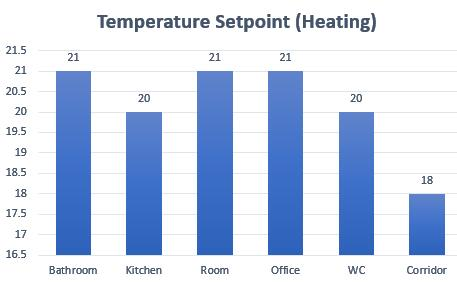
\includegraphics[scale=1]{TempSetpoint.jpg}
			\caption{Heating Temperature Set point}
			\label{fig:HeatingSP}
			\end{figure}
			

			\begin{figure}[h!]
			\centering
			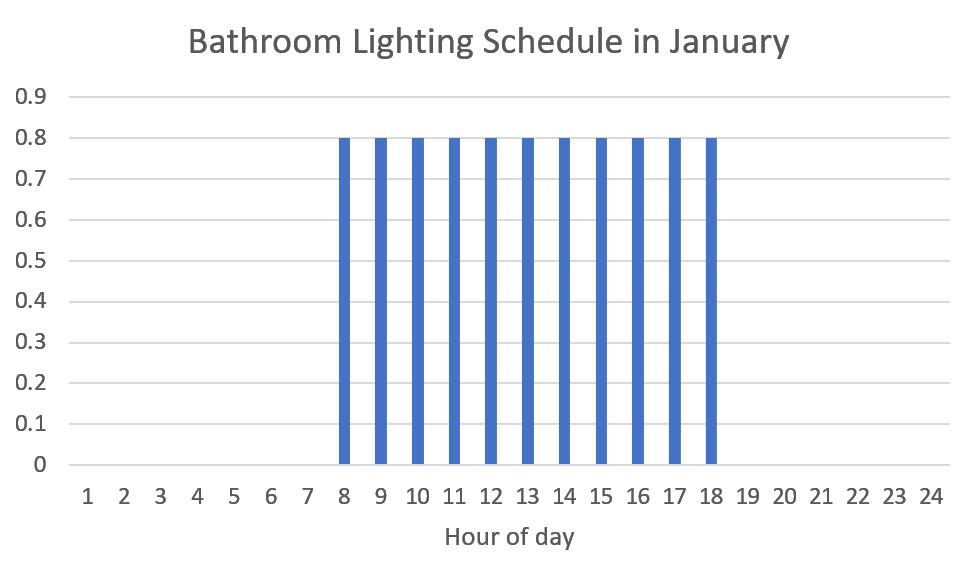
\includegraphics[scale=0.4]{JanBath_Light.jpg}
			\caption{Bathroom Lighting Schedule in January}
			\label{fig:JanBathLight}
			\end{figure}
			



	\subsection{Calibration}
		In order to ensure the simulated buildings have similar thermal behaviors as the real buildings, a calibration to the building envelope is needed. The calibration process needs to be in a summer period where no heating and cooling is performed. The calibration process vary the building air tightness, internal loads, and user behaviors until the calculated indoor temperature behaves similar enough to the historical measurement. Lastly, the calibrated building is again subject to annual analysis and aim to match the calculated annual energy consumption with the actual measured value.
		

		\subsubsection{Building Envelope Calibration}
			The air tightness is thought to be an important factor in building simulation. Therefore, the calibration process would vary the air tightness between 0.1 to 0.5 ach and try to match both the hourly indoor temperature as well as the annual heating demand.

		\subsubsection{Internal Loads}
			Internal load such as Lighting and appliance schedule can change the indoor temperature patten. Therefore, in the calibration process, lighting schedule and electricity schedule are modified to observe the indoor temperature of the focused un-heating period. The newly constructed schedules should be separated into weekday and weekend schedule.

		\subsubsection{User behavior}
			The user behavior is also thought to be an influential factor to indoor comfort. The calibration also investigate the control strategies for users to operate the window shading. A number of shading control is used and the strategy with most similar indoor temperature patten is used in the calibrated model. The newly constructed shading schedule should vary between summer and winter schedule.


	\subsection{Parameters Variation}
		After the building model has been constructed and calibrated, a further analysis with varied parameters can be performed. Here are the parameters that are focused and subject to variation:\\
		\begin{itemize}
			\item Heating temperature setpoint for all zones
			\item Occupancy schedule for kay zones (except toilet, wc and corridor)
			\item appliance schedule for all zones (Lighting, Electricity, Domestic hot water)
			\item Ventilation level for all zones
			\item Air infiltration
			\item Internal convection coefficient
			\item External convection coefficient
			\item Facade solar absorptance\\
		\end{itemize}
		
		\textit{jE-Plus}\\
		\textit{jE-Plus} is used as a tool to process the parameter variation analysis. It allows a number of preset parameters to replace certain values in the EnergyPlus file, and allow parallel  There are one thousand building samples with random combination of parameters. \\


		\textit{Heating Temperature Setpoint}\\
			All zones' heating setpoint temperature are part of the parameter variation. The heating setpoint temperature for the same category at the same floor are thought to be identical. For example, the heating setpoint temperature of \textit{Room2} and \textit{Room3} at the second floor would be the same, but might be different to the heating setpoint temperatues for \textit{Room2} and \textit{Room3} at third floor.\\
			The range of temperature setpoints for each zones is shown in Figure \ref{fig:TempSetpoint} below. The temperature setpoint is randomly created in a normal distribution between a pre-set range.\\

			\begin{figure}[H]
			\centering
			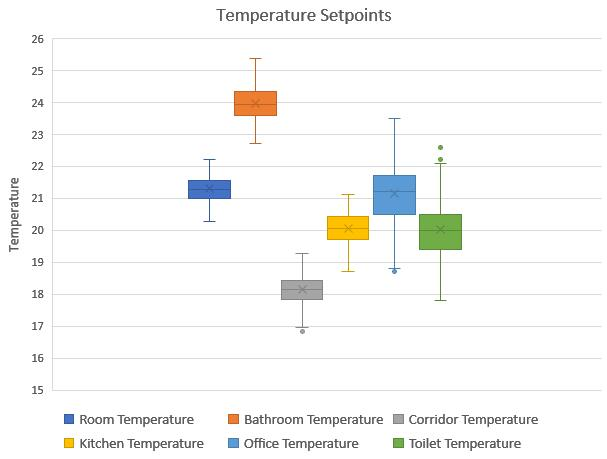
\includegraphics[scale=0.8]{Residential_TempSetpoint.jpg}
			\caption{Heating Temperature Setpoint Distribution}
			\label{fig:TempSetpoint}
			\end{figure}
			
		\textit{Ventilation Level}\\
			Similarly, the ventilation level for each zone is given in Figure \ref{fig:VentLevel} below. The ventilation level for the same zone category at the same floor are thought to be identical. The ventilation level vary according to a normal distribution rule as shown in Figure \ref{fig:VentDist} below.\\
			\begin{figure}[H]
			\centering
			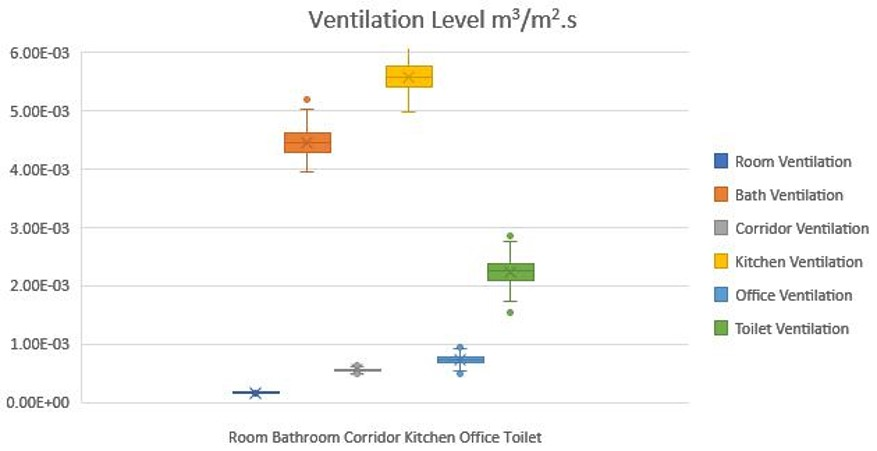
\includegraphics[scale=0.55]{VentilationLevel.jpg}
			\caption{Ventilation Level Distribution}
			\label{fig:VentLevel}
			\end{figure}

			\begin{figure}[H]
			\centering
			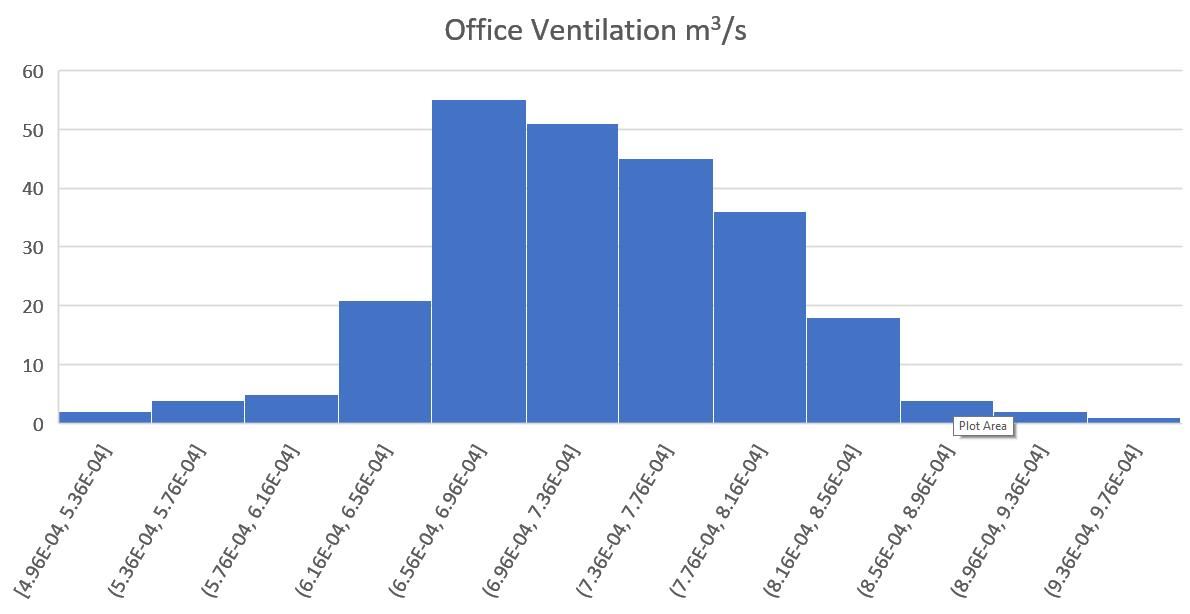
\includegraphics[scale=0.55]{Office_Vent.jpg}
			\caption{Air Ventilation Distribution}
			\label{fig:VentDist}
			\end{figure}
			
			
		\textit{Infiltration}\\
			The infiltration level is roughly a normal distribution which takes $\pm$ 10\% of the calibrated value as its standard deviation. Figure \ref{fig:EXPAirInfiltration_Sumatra} below shows an example air infiltration distribution.\\

			\begin{figure}[H]
			\centering
			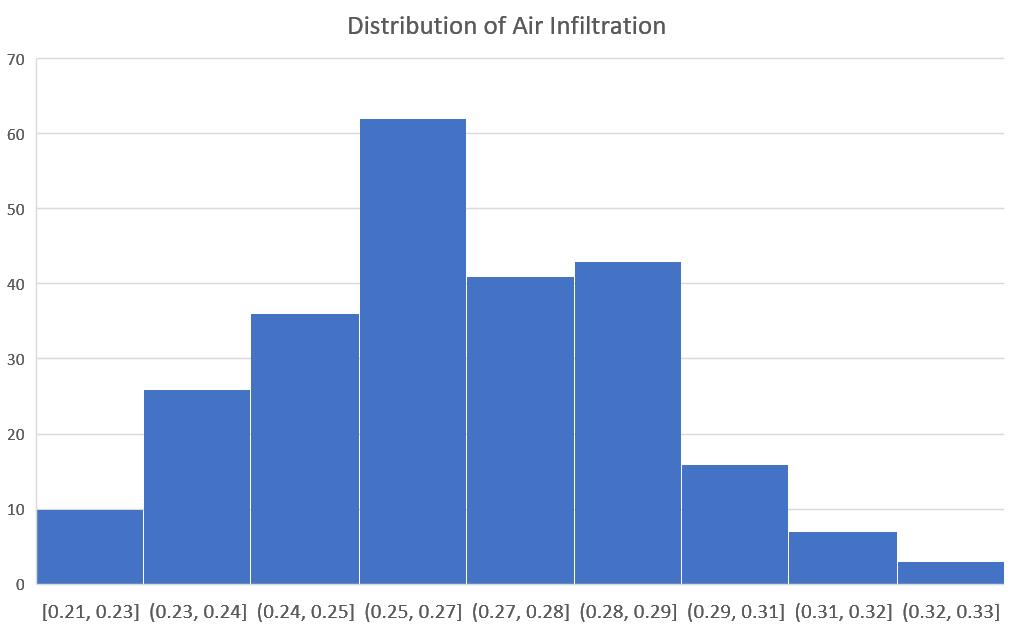
\includegraphics[scale=0.5]{Example_Normal_Distribution.jpg}
			\caption{Example Air Infiltration Distribution}
			\label{fig:EXPAirInfiltration_Sumatra}
			\end{figure}
		
		\textit{Internal and External convection coefficient}\\
			The internal and external convection coefficient range between $\pm 10\%$ of the nominal value.
			A discrete distribution is applied, means the probability of the convection coefficient being any number between $\pm 10\%$ of the nominal value is the same. Figure xx and Figure below shows a distribution histogram of the internal and external heat convection coefficient.\\

			\begin{figure}[H]
			\centering
			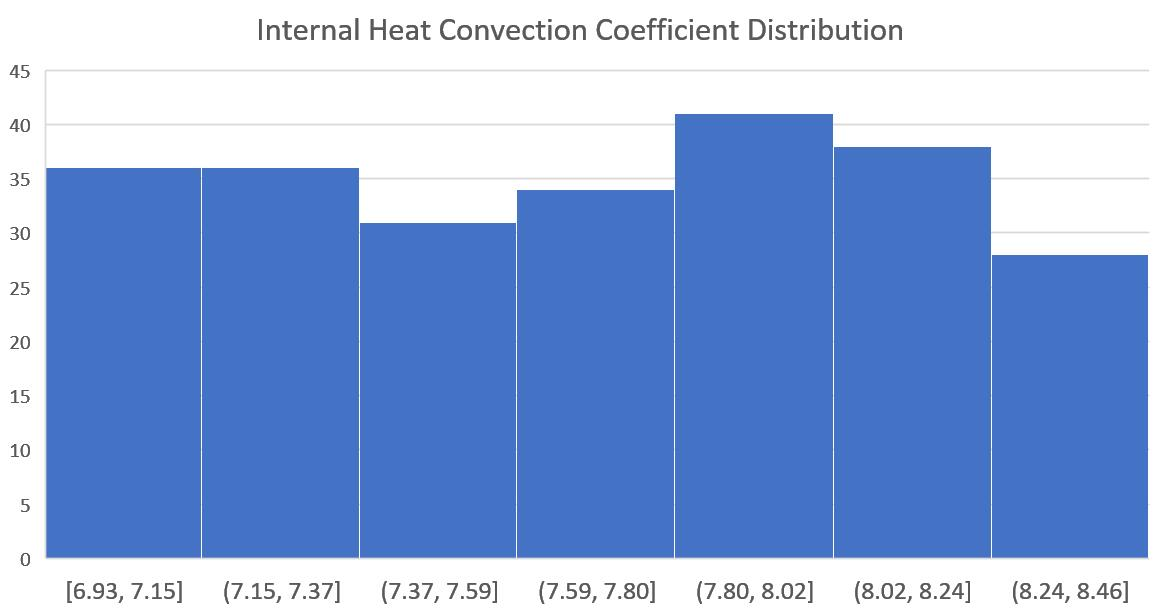
\includegraphics[scale=0.5]{Hongger_InConvDist.jpg}
			\caption{Internal Heat Convection Coefficient Distribution}
			\label{fig:HonggerIntConvDist}
			\end{figure}
			
			\begin{figure}[H]
			\centering
			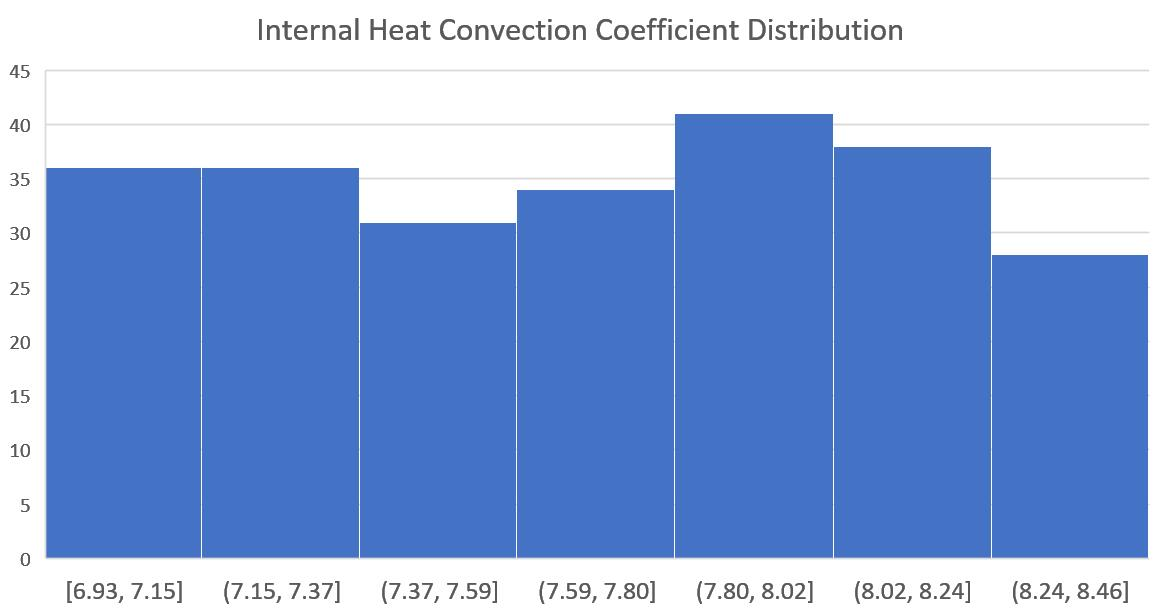
\includegraphics[scale=0.5]{Hongger_InConvDist.jpg}
			\caption{External Heat Convection Coefficient Distribution}
			\label{fig:HonggerExtConvDist}
			\end{figure}
			

		\textit{Facade solar absorptance}\\
			The facade paint and facade color determine the facade solar absorptance. It range from 0 to 1 where a 0 absorptance means the surface reflex all the energy onto the surface, and a 1 absorptance means the facade absorb all the solar energy onto the surface. In this analysis the solar absorptance vary between 0.2 to 0.9 at a discrete distribution.
	
	\subsection{Data Processing}
		\textit{Python} and Excel are used process the results, where excel is used to generate histograms and other regular charts, while Python (with Matplotlib package) is used to merge data sets, process a series of data files, generate other irregular charts such as correlation matrix, and some boxplots.

		\subsubsection{Dynamic Analysis Range}
			Histogram and boxplots are used to show the distribution and the range to the dynamic analysis results after the parameter variation. A box is focus on the effect of different simulation environments or parameters while a histogram focus more on the range and the distribution of a single variable.

		\subsubsection{Correlation Matrix}
			In order to display the relations between parameters and the relations between parameters and heating demands and DHW demands, a correlation matrix is needed to show their influence on each other. \\
			Essentially, the correlation matrix is a heat map matrix where a deeper color represent a higher absolute value. Correlation range between -1 to 1, where -1 and 1 represent a perfect linear relationship and 0 indicates that there is no association between two variables.\\
		


\newpage
\section{Results}

	\subsection{Static Calculation}
		The results of static calculation are shown in the following sections. Firstly the results of office building then the residential building results at each steps are shown below according the methodology. A summary is also given after each energy loss and energy gain section is presented.

		\subsubsection{Summary of Results}

		\begin{figure}[H]
		\centering
		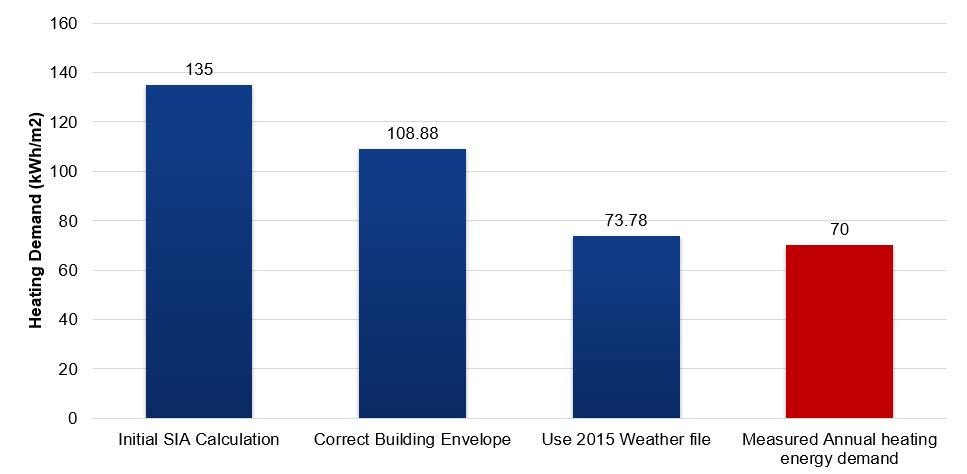
\includegraphics[scale=0.4]{Office_SIA.jpg}
		\caption{SIA Calculation Improvement for Office Building}
		\label{fig:Sumatra_SIA}
		\end{figure}
		
		\begin{figure}[h!]
		\centering
		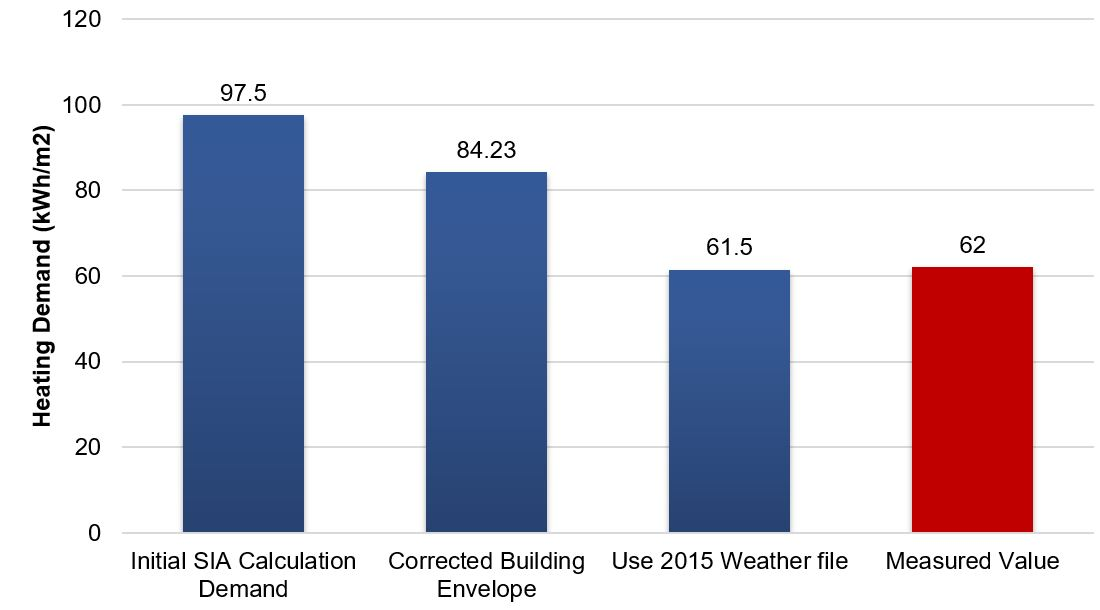
\includegraphics[scale=0.4]{Residential_SIA.jpg}
		\caption{SIA Calculation Improvement for Residential Building}
		\label{fig:Hongger_SIA}
		\end{figure}
		
		
		Compare the results
			\begin{itemize}
			 	\item Previous Result (by Lemon Consult)
			 	\item Apply correct building floor and wall area
			 	\item Apply year 2015 weather data
			 	\item Modify air tightness (infiltration)
			 	\item Historical measurement value
			 \end{itemize}
			  
		\subsubsection{EnergyPlus Simulation Result}		
		\begin{itemize}
			\item Floor Area (be used in SIA calculation)
			\item Heating Demand
			\item Air Ventilation
		\end{itemize}
		The first set of dynamic analysis (4 sets of heating demand distribution from infiltration 0.1 to 0.4)

		\begin{figure}[H]
		\centering
		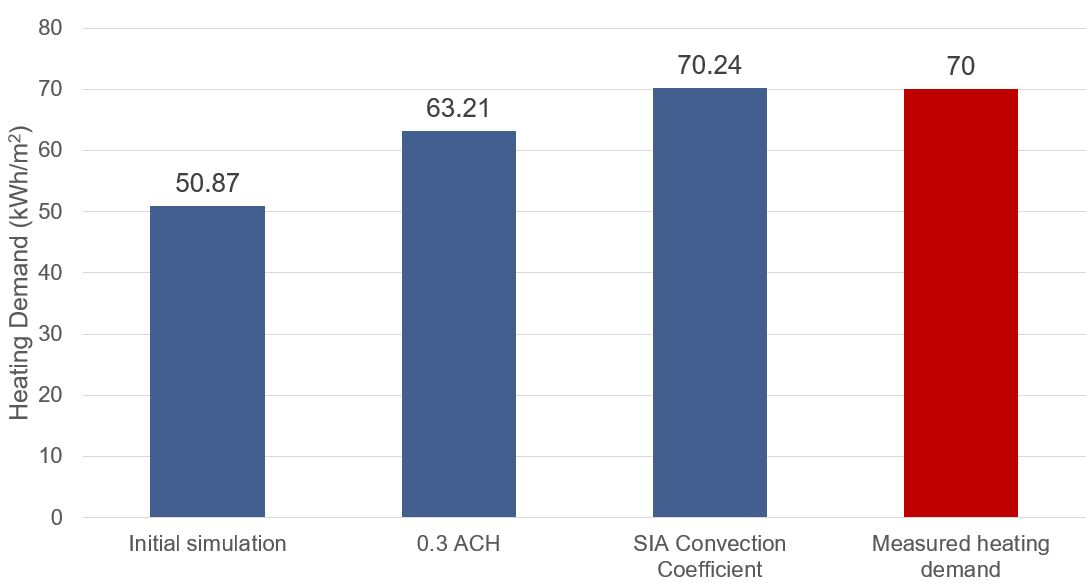
\includegraphics[scale=0.5]{Office_EP.jpg}
		\caption{Office Building Dynamic Calculation Correction}
		\label{fig:Sumatra_EP}
		\end{figure}

		\begin{figure}[h!]
		\centering
		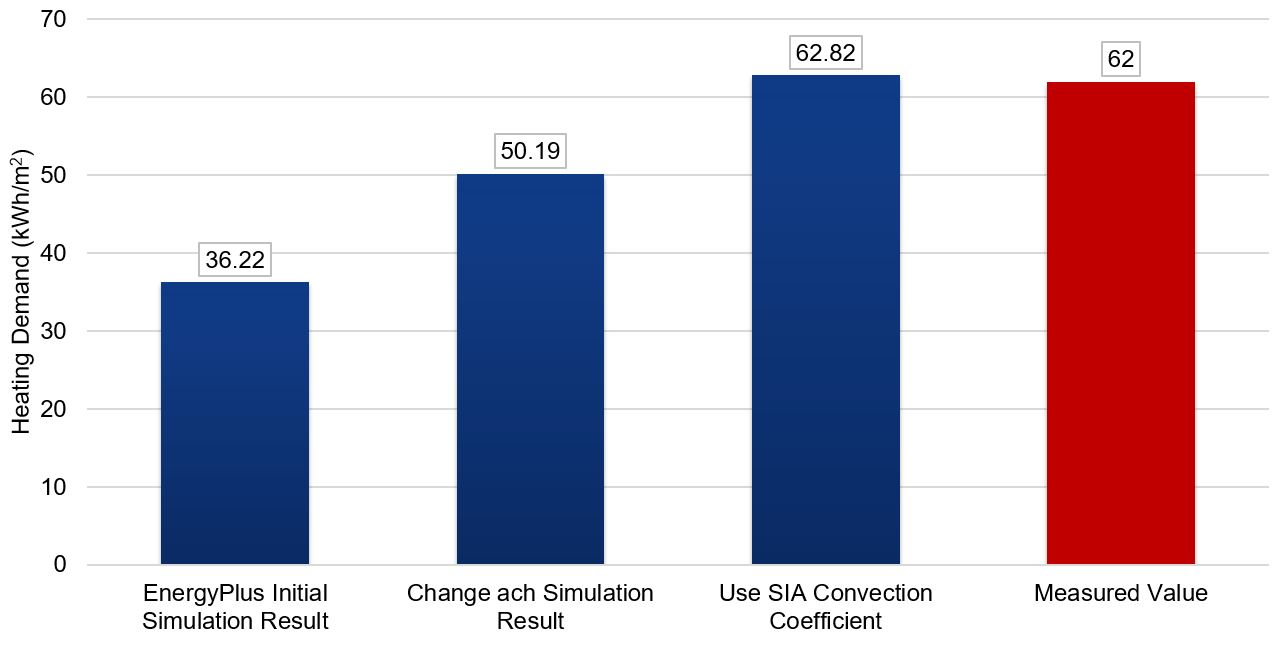
\includegraphics[scale=0.5]{Residential_EP.jpg}
		\caption{Residential Building Dynamic Calculation Correction}
		\label{fig:Hongger_EP}
		\end{figure}
		
		




		\subsubsection{Calibration Results}
			\begin{itemize}
				\item Steps of calibration (hourly - annually)
				\item Outdoor temperature compare
				\item Results of the calibration
				\item Final Calibrated Settings
			\end{itemize}
			
		\subsubsection{Parameters Variation Results}
			\begin{itemize}
				\item Dynamic Heating Demand Variation
				\item Dynamic DHW Demand Variation
				\item Results of all parameters (range and distribution of heating demand and DHW demand)
				\item Correlation of parameters
			\end{itemize}


		\subsubsection{Effect of Convection Coefficient on Heating Demand}
        	As the correlation matrix above indicated week correlation between heating demand and heat convection coefficients, another set of simulation with 100 extra samples are processed. These samples are modified from the calibrated building model, with the only difference in convection coefficient (ranging from 90\% to 110\% of the calibrated values). The results are shown in the graphs below.
        \subsubsection{Effect of Solar Absorptance on Heating Demand}
			Similarly, an extra set of samples with different solar absorptance are processed in jE-Plus.

\newpage
\section{Discussion}

		\begin{itemize}
		\item Key parameters (Which parameters are the most important and which are not as important)
		\item Key assumptions (Are these assumption still applicable)
		\item Recommendation (building envelope much be accurate, a weather data update is critical etc)
	\end{itemize}






\newpage			
\section{Conclusion}
	\begin{itemize}
		\item Key parameters
		\item Recommended set of parameters
		\item General Recommendations
	\end{itemize}


%\section{Reference}
\newpage
\printbibliography



\section{Appendix}
\subsection{Assumptions}

	\textit{Adiabatic Walls}\\
	As the residential building is attached to other buildings on both sides, the two walls that attach other buildings are seen as adiabatic. Similarily, as the north facade of the office building is attached to another building, it is also seen as adiabatic wall.\\

	\textit{No underground warehouses}\\
	The cellar of the residential building is not considered in this thesis and assume a constant temperature of 18 degree environment attach the ground floor.\\

	\textit{Ignore the tilted roof and loft}\\
	Due to lack of information about the internal layout of the top floor, the tilted roof and the loft of the residential building is represented as a regular size floor with exactly the same layout as the first floor.\\

	\textit{Ignore the vegitation covering}\\
	The majority part of the northen and the easten facade of the office building as well as both external walls of the residential building are covered with plants. However, as the effect of vegitation covering is unknow, the vegitation layer of these facade is ignored in the modeling and analysis process.\\


\subsection{TARP Algorithm for convection coefficient}
\[h_c = h_f + h_n\]
\[h_f = 2.537 W_f R_f \left(\frac{PV_z}{A}\right)^\frac{1}{2}\]


\[W_f = 1  \text{   Windward surface}\]
\[W_f = 0.5 \text{   Leeward surface}\]

\[R_f = 1.67 \text{: Brick}\]
\[R_f = 1.52 \text{: Concrete}\]
\[R_f = 1.13 \text{: Clear pine}\]
\[R_f = 1 \text{: glass}\]
\[h_n = 1.31 | \Delta T|^{1/3}\]
for vertical surface


\subsection{Detailed SIA Calculation}
	
		
	\subsubsection{Residential Building Heating Demand}
		
		\textbf{Transmission Heat Loss}\\
		Table \ref{tab:HonggTransmission} below show a the transmission heat loss for each building element under both SIA 381/2 weather data and the 2015 weather station data. The unit of heat loss is in MJ/m$^2$.
				% Table generated by Excel2LaTeX from sheet 'Sheet1'
		\begin{table}[htbp]
		\small
		\centering
		\caption{Heat Transmission Heat Loss of Residential Building}
		    \begin{tabular}{|ccccc|}
		    \toprule
		    \multicolumn{5}{|c|}{\textbf{Heat Transmission Loss}} \\
		    \midrule
		          & \multicolumn{1}{p{4.785em}}{Area m2} & \multicolumn{1}{p{4.785em}}{U-Value W/m2.K} & \multicolumn{1}{p{5.715em}}{Loss (SIA) MJ/m2} & \multicolumn{1}{p{5.715em}|}{Loss(2015) MJ/m2} \\
		    \midrule
		    Outside Wall & 208.6088 & 1.006 & 152.60 & 117.63 \\
		    Window FE-EG-1a & 9.9   & 2.379 & 17.13 & 13.21 \\
		    Window FE-EG-2a & 26    & 2.388 & 45.16 & 34.82 \\
		    Window FE-EG-3a & 3     & 2.19  & 4.78  & 3.68 \\
		    Window FE-EG-4a & 20.8  & 2.285 & 34.57 & 26.65 \\
		    Window FE-TH-1a & 3.7   & 2.33  & 6.27  & 4.83 \\
		    Door Tur-TH & 2.5   & 3.5   & 6.36  & 4.91 \\
		    Ceiling & 101.2115 & 1.6145418 & 37.92 & 31.90 \\
		    Ground floor & 101.2115 & 1.3504216 & 31.72 & 26.69 \\
		    \midrule
		    Total &       &       & 336.52 & 264.32 \\
		    \bottomrule
		    \end{tabular}%
		  \label{tab:HonggTransmission}%
		\end{table}%

		\textbf{Ventilation Heat Loss}\\
		Table \ref{tab:HonggVentLoss380} below shows the monthly and the annual ventilation heat loss per $m^2$ of floor area under monthly SIA 382/1 weather data and 2015 Zurich weather station data. Similarly, the energy loss is in MJ/m$^2$.\\
		% Table generated by Excel2LaTeX from sheet 'Sheet1'
		\begin{table}[H]
		\centering
		\small
		\caption{Residential Building Ventilation Heat Loss}
		    \begin{tabular}{|p{6.855em}ccccccccccccc|}
		    \toprule
		    \multicolumn{14}{|c|}{Ventilation Heat Loss MJ/m2} \\
		    \midrule
		    \multicolumn{1}{|c}{Month} & Jan  & Feb  & Mar  & Apr  & May  & Jun  & Jul  & Aug  & Sep  & Oct  & Nov  & Dec  & Sum \\
		    \midrule
		    Heating Degree Days (2015) & 498  & 519  & 344  & 149  & 30.6 & 0    & 0    & 0    & 17.8 & 225  & 268  & 462  & 2513 \\
		    Heating Degree Days (SIA) & 615  & 501  & 467  & 255  & 110  & 23   & 7    & 6    & 35   & 207  & 433  & 601  & 3260 \\
		    Ventilation Loss SIA & 12   & 9.76 & 9.1  & 4.97 & 2.14 & 0.45 & 0.14 & 0.12 & 0.68 & 4.03 & 8.44 & 11.7 & 63.53 \\
		    Ventilation Heat loss 2015 & 9.71 & 10.1 & 6.7  & 2.9  & 0.6  & 0    & 0    & 0    & 0.35 & 4.38 & 5.23 & 9    & 48.98 \\
		    \bottomrule
		    \end{tabular}%

		  \label{tab:HonggVentLoss380}%
		\end{table}%

		\textbf{Heat Loss Through Thermal Bridge}\\
		The heat loss through thermal bridge of all building elements are shown below in Table \ref{tab:HonggerThermalBridge} below.
		\begin{table}[H]
		\small
		\centering
		\caption{Thermal Bridge Calculation For Residential Building}
		    \begin{tabular}{ccrccccc}
		    \toprule
		    \multicolumn{1}{l}{Nr.} & \multicolumn{2}{c}{Component} & Lost Coefficient & Length & H(U*A*b) & SIA 381/2 & 2015 Zurich \\
		         &      &      & W/mK & m    & W/K  & MJ/m2 & MJ/m2 \\
		    \midrule
		    1    & \multicolumn{1}{r}{Tür-TH} & \multicolumn{1}{l}{(Sturz)} & 0.1  & 1    & 0.1  & 0.07323747 & 0.056459083 \\
		    2    & \multicolumn{1}{r}{Tür-TH} & \multicolumn{1}{l}{(Brüstung)} & 0.1  & 1    & 0.1  & 0.07323747 & 0.056459083 \\
		    3    & \multicolumn{1}{r}{Tür-TH} & \multicolumn{1}{l}{(Leibung)} & 0.1  & 5    & 0.5  & 0.36618737 & 0.282295415 \\
		    4    & \multicolumn{1}{r}{FE-EG-1a} & \multicolumn{1}{l}{(Sturz)} & 0.1  & 3.6  & 0.36 & 0.26365491 & 0.203252699 \\
		    5    & \multicolumn{1}{r}{FE-EG-1a} & \multicolumn{1}{l}{(Brüstung)} & 0.1  & 3.6  & 0.36 & 0.26365491 & 0.203252699 \\
		    6    & \multicolumn{1}{r}{FE-EG-1a} & \multicolumn{1}{l}{(Leibung)} & 0.1  & 5.8  & 0.58 & 0.42477735 & 0.327462681 \\
		    7    & \multicolumn{1}{r}{FE-EG-2a} & \multicolumn{1}{l}{(Sturz)} & 0.1  & 10   & 1    & 0.73237474 & 0.56459083 \\
		    8    & \multicolumn{1}{r}{FE-EG-2a} & \multicolumn{1}{l}{(Brüstung)} & 0.1  & 10   & 1    & 0.73237474 & 0.56459083 \\
		    9    & \multicolumn{1}{r}{FE-EG-2a} & \multicolumn{1}{l}{(Leibung)} & 0.1  & 52   & 5.2  & 3.80834863 & 2.935872315 \\
		    10   & \multicolumn{1}{r}{FE-EG-3a} & \multicolumn{1}{l}{(Sturz)} & 0.1  & 2.5  & 0.25 & 0.18309368 & 0.141147707 \\
		    11   & \multicolumn{1}{r}{FE-EG-3a} & \multicolumn{1}{l}{(Brüstung)} & 0.1  & 2.5  & 0.25 & 0.18309368 & 0.141147707 \\
		    12   & \multicolumn{1}{r}{FE-EG-3a} & \multicolumn{1}{l}{(Leibung)} & 0.1  & 12   & 1.2  & 0.87884968 & 0.677508996 \\
		    13   & \multicolumn{1}{r}{FE-EG-4a} & \multicolumn{1}{l}{(Sturz)} & 0.1  & 13   & 1.3  & 0.95208716 & 0.733968079 \\
		    14   & \multicolumn{1}{r}{FE-EG-4a} & \multicolumn{1}{l}{(Brüstung)} & 0.1  & 13   & 1.3  & 0.95208716 & 0.733968079 \\
		    15   & \multicolumn{1}{r}{FE-EG-4a} & \multicolumn{1}{l}{(Leibung)} & 0.1  & 41.6 & 4.16 & 3.0466789 & 2.348697852 \\
		    16   & \multicolumn{1}{r}{FE-TH-1a} & \multicolumn{1}{l}{(Sturz)} & 0.1  & 3.68 & 0.37 & 0.27097865 & 0.208898607 \\
		    17   & \multicolumn{1}{r}{FE-TH-1a} & \multicolumn{1}{l}{(Brüstung)} & 0.1  & 3.68 & 0.37 & 0.27097865 & 0.208898607 \\
		    18   & \multicolumn{1}{r}{FE-TH-1a} & \multicolumn{1}{l}{(Leibung)} & 0.1  & 7.8  & 0.78 & 0.57125229 & 0.440380847 \\
		    \midrule
		    \multicolumn{3}{c}{Total} &     & 191.8 &            & 14.05 & 10.83 \\
		    \bottomrule
		    \end{tabular}%
		  \label{tab:HonggerThermalBridge}%
		\end{table}%

		\textbf{Internal Gains by Occupants}\\ 
		% Table generated by Excel2LaTeX from sheet 'Sheet1'
		\begin{table}[htbp]
		\centering
		\caption{Internal Gains by Occupants in Residential Building}
		    \begin{tabular}{cccc}
		    \toprule
		    \multicolumn{4}{c}{Internal Gains by person} \\
		    \midrule
		    \multicolumn{1}{p{8.07em}}{Occupancy m2/P} & \multicolumn{1}{p{7em}}{Unit Gain W/P} & \multicolumn{1}{p{7.355em}}{Present hour } & \multicolumn{1}{p{7.355em}}{Gain (MJ/m2)} \\
		    40    & 70    & 12    & 27.594 \\
		    \bottomrule
		    \end{tabular}%
		  \label{tab:HonggOccupancyGain}%
		\end{table}%

		\textbf{Internal Gains by Electronics}\\
		\begin{table}[htbp]
		\centering
		\caption{Heat Gain by Electronics in Residential Building}
		    \begin{tabular}{ccccc}
		    \toprule
		    \multicolumn{5}{c}{Internal Gains by electronics} \\
		    \midrule
		    \multicolumn{1}{p{5.355em}}{Weather data} & \multicolumn{1}{p{5.355em}}{Unit demand (kWh/m2)} & \multicolumn{1}{p{5.355em}}{Factor} & \multicolumn{1}{p{5.355em}}{Heating Day} & \multicolumn{1}{p{5.355em}}{Heat Gain (MJ/m2)} \\
		    2015  & 28    & 0.7   & 175   & 33.83 \\
		    SIA   & 28    & 0.7   & 208   & 40.21 \\
		    \bottomrule
		    \end{tabular}%
		  \label{tab:HonggElecGain}%
		\end{table}%

		\textbf{Internal Gains by Solar Radiation}\\
		\begin{table}[htbp]
		\centering
		\small
		\caption{Solar Gains in Residential Building}
		    \begin{tabular}{lrrrrrrrrrrr}
		    \toprule
		    \multicolumn{12}{c}{Solar Gains ($MJ/m^2$)} \\
		    \midrule
		    \multicolumn{1}{p{4.215em}}{Window Names} & \multicolumn{1}{c}{Orient} & \multicolumn{1}{c}{Area} & \multicolumn{1}{c}{f1} & \multicolumn{1}{c}{f2} & \multicolumn{1}{c}{f3} & \multicolumn{1}{c}{fg} & \multicolumn{1}{c}{g} & \multicolumn{1}{p{4.57em}}{Radiation\newline{}SIA} & \multicolumn{1}{p{4.57em}}{Radiation\newline{}2015} & \multicolumn{1}{p{3.8em}}{Solar Gain (SIA)} & \multicolumn{1}{p{3.8em}}{Solar Gain (2015)} \\
		    \midrule
		    FE-EG-1a & \multicolumn{1}{l}{NE} & 6.9   & 0.89  & 0.97  & 0.99  & 0.64  & 0.5   & 1563.92 & 1388.59 & 7.62  & 6.77 \\
		    FE-EG-2a & \multicolumn{1}{l}{NE} & 10.4  & 0.89  & 0.97  & 0.99  & 0.53  & 0.5   & 1563.92 & 1388.59 & 9.51  & 8.45 \\
		    FE-EG-2a & \multicolumn{1}{l}{SW} & 15.6  & 0.82  & 0.97  & 0.98  & 0.53  & 0.5   & 2653.31 & 2683.81 & 22.08 & 22.34 \\
		    FE-EG-3a & \multicolumn{1}{l}{SW} & 3     & 0.82  & 0.97  & 0.98  & 0.3   & 0.5   & 2653.31 & 2683.81 & 2.40  & 2.43 \\
		    FE-EG-4a & \multicolumn{1}{l}{NE} & 14.4  & 0.89  & 0.97  & 0.99  & 0.5   & 0.5   & 1563.92 & 1388.59 & 12.43 & 11.03 \\
		    FE-EG-4a & \multicolumn{1}{l}{SW} & 6.4   & 0.82  & 0.97  & 0.98  & 0.5   & 0.5   & 2653.31 & 2683.81 & 8.55  & 8.64 \\
		    FE-TH-1a & \multicolumn{1}{l}{NE} & 2.88  & 0.89  & 0.97  & 0.99  & 0.54  & 0.5   & 1563.92 & 1388.59 & 2.68  & 2.38 \\
		    FE-TH-1a & \multicolumn{1}{l}{SW} & 2.8   & 0.82  & 0.97  & 0.98  & 0.54  & 0.5   & 2653.31 & 2683.81 & 4.04  & 4.08 \\
		    \midrule
		    Total &       &       &       &       &       &       &       &       &       & 69.32 & 66.13 \\
		    \bottomrule
		    \end{tabular}%
		  \label{tab:HonggSolarGain}%
		\end{table}%

		\subsubsection{Office Building Calculation Results}

		\textbf{Transmission Heat Loss}\\
		% Table generated by Excel2LaTeX from sheet 'Sheet1'
		\begin{table}[H]
		\centering
		\caption{Transmission Heat Loss of Office Building}
		    \begin{tabular}{crrrr}
		    \toprule
		    \multicolumn{5}{c}{Heat Transmission Loss $MJ/m^2$} \\
		    \midrule
		          & \multicolumn{1}{p{4.215em}}{Area} & \multicolumn{1}{p{4.215em}}{U-Value} & \multicolumn{1}{p{4.215em}}{Loss \newline{}(SIA) } & \multicolumn{1}{p{4.215em}}{Loss (2015)} \\
		    \midrule
		    Earth Wall East & \multicolumn{1}{c}{121.73} & \multicolumn{1}{c}{3.47} & \multicolumn{1}{c}{143.92} & \multicolumn{1}{c}{110.94} \\
		    External Wall East & \multicolumn{1}{c}{110.34} & \multicolumn{1}{c}{0.96} & \multicolumn{1}{c}{36.16} & \multicolumn{1}{c}{27.88} \\
		    Outside Wall Other & \multicolumn{1}{c}{159.35} & \multicolumn{1}{c}{1.37} & \multicolumn{1}{c}{74.43} & \multicolumn{1}{c}{57.38} \\
		    Window FE1 & \multicolumn{1}{c}{198.00} & \multicolumn{1}{c}{2.00} & \multicolumn{1}{c}{134.98} & \multicolumn{1}{c}{104.05} \\
		    Window FE2 & \multicolumn{1}{c}{8.13} & \multicolumn{1}{c}{2.50} & \multicolumn{1}{c}{6.92} & \multicolumn{1}{c}{5.33} \\
		    Window FE3 & \multicolumn{1}{c}{2.70} & \multicolumn{1}{c}{2.50} & \multicolumn{1}{c}{2.30} & \multicolumn{1}{c}{1.77} \\
		    Window FE4 & \multicolumn{1}{c}{10.50} & \multicolumn{1}{c}{2.05} & \multicolumn{1}{c}{7.32} & \multicolumn{1}{c}{5.65} \\
		    Window FE5 & \multicolumn{1}{c}{7.79} & \multicolumn{1}{c}{2.07} & \multicolumn{1}{c}{5.50} & \multicolumn{1}{c}{4.24} \\
		    Window FE6 & \multicolumn{1}{c}{4.50} & \multicolumn{1}{c}{2.03} & \multicolumn{1}{c}{3.11} & \multicolumn{1}{c}{2.40} \\
		    Window FE7 & \multicolumn{1}{c}{5.76} & \multicolumn{1}{c}{2.04} & \multicolumn{1}{c}{4.01} & \multicolumn{1}{c}{3.09} \\
		    Window FE8 & \multicolumn{1}{c}{2.93} & \multicolumn{1}{c}{1.91} & \multicolumn{1}{c}{1.90} & \multicolumn{1}{c}{1.47} \\
		    Ceiling & \multicolumn{1}{c}{231.96} & \multicolumn{1}{c}{0.88} & \multicolumn{1}{c}{69.39} & \multicolumn{1}{c}{53.49} \\
		    Ground floor & \multicolumn{1}{c}{231.96} & \multicolumn{1}{c}{1.90} & \multicolumn{1}{c}{38.32} & \multicolumn{1}{c}{32.24} \\
		    \midrule
		    Total &       &       & 528.26 & 409.92 \\
		    \bottomrule
		    \end{tabular}%
		  \label{tab:SumatraTransmission Loss}%
		\end{table}%


		\textbf{Ventilation Heat Loss}\\
% Table generated by Excel2LaTeX from sheet 'Sheet1'
\begin{table}[H]
  \centering
  \small
  \caption{Ventilation Heat Loss of Office Building}
    \begin{tabular}{|p{4.5em}rrrrrrrrrrrrr|}
    \toprule
    \multicolumn{14}{|c|}{Ventilation Heat Loss (MJ/m2)} \\
    \midrule
    \multicolumn{1}{|l}{ } & \multicolumn{1}{l}{Jan} & \multicolumn{1}{l}{Feb} & \multicolumn{1}{l}{Mar} & \multicolumn{1}{l}{Apr} & \multicolumn{1}{l}{May} & \multicolumn{1}{l}{Jun} & \multicolumn{1}{l}{Jul} & \multicolumn{1}{l}{Aug} & \multicolumn{1}{l}{Sep} & \multicolumn{1}{l}{Oct} & \multicolumn{1}{l}{Nov} & \multicolumn{1}{l}{Dec} & \multicolumn{1}{l|}{Sum} \\
    \midrule
    \multicolumn{1}{|l}{HDD 2015} & 498.3 & 518.9 & 343.8 & 148.6 & 30.6 & 0.0  & 0.0  & 0.0  & 17.8 & 224.9 & 268.3 & 461.9 & 2513.15 \\
    \multicolumn{1}{|l}{HDD SIA} & 615.0 & 501.0 & 467.0 & 255.0 & 110.0 & 23.0 & 7.0  & 6.0  & 35.0 & 207.0 & 433.0 & 601.0 & 3260.00 \\
    Ventilation Loss 2015 & 9.71 & 10.11 & 6.70 & 2.90 & 0.60 & 0.00 & 0.00 & 0.00 & 0.35 & 4.38 & 5.23 & 9.00 & 48.98 \\
    Ventilation Loss SIA & 11.99 & 9.76 & 9.10 & 4.97 & 2.14 & 0.45 & 0.14 & 0.12 & 0.68 & 4.03 & 8.44 & 11.71 & 63.53 \\
    \bottomrule
    \end{tabular}%
  \label{tab:SumatraVentLoss}%
\end{table}%


		\textbf{Heat Loss Through Thermal Bridge}\\

% Table generated by Excel2LaTeX from sheet 'Sheet2'
\begin{table}[H]
\centering
\small
\caption{Thermal Bridge Heat Loss in Office Building}
    \begin{tabular}{ccccrrr}
    \toprule
    \multicolumn{7}{c}{Thermal Bridge Loss in Office Building ($MJ/m^2$)} \\
    \hline
    \multicolumn{3}{c}{Code} & \multicolumn{1}{p{2.785em}}{$\Psi$} & \multicolumn{1}{c}{Length\newline{} m} & \multicolumn{1}{p{3em}}{Loss (SIA)} & \multicolumn{1}{p{3em}}{Loss (2015)} \\
    \multicolumn{1}{l}{FE} & \multicolumn{1}{r}{1} & \multicolumn{1}{l}{(Sturz)} & \multicolumn{1}{r}{0.5} & 99   & 16.864 & 11.772 \\
    \multicolumn{1}{l}{FE} & \multicolumn{1}{r}{1} & \multicolumn{1}{l}{(Brüstung)} & \multicolumn{1}{r}{0.5} & 99   & 16.864 & 11.772 \\
    \multicolumn{1}{l}{FE} & \multicolumn{1}{r}{1} & \multicolumn{1}{l}{(Leibung)} & \multicolumn{1}{r}{0.5} & 132  & 22.486 & 15.696 \\
    \multicolumn{1}{l}{FE} & \multicolumn{1}{r}{2} & \multicolumn{1}{l}{(Sturz)} & \multicolumn{1}{r}{0.5} & 3    & 0.511 & 0.357 \\
    \multicolumn{1}{l}{FE} & \multicolumn{1}{r}{2} & \multicolumn{1}{l}{(Brüstung)} & \multicolumn{1}{r}{0.5} & 3    & 0.511 & 0.357 \\
    \multicolumn{1}{l}{FE} & \multicolumn{1}{r}{2} & \multicolumn{1}{l}{(Leibung)} & \multicolumn{1}{r}{0.5} & 5.4  & 0.920 & 0.642 \\
    \multicolumn{1}{l}{FE} & \multicolumn{1}{r}{3} & \multicolumn{1}{l}{(Sturz)} & \multicolumn{1}{r}{0.5} & 1.35 & 0.230 & 0.161 \\
    \multicolumn{1}{l}{FE} & \multicolumn{1}{r}{3} & \multicolumn{1}{l}{(Brüstung)} & \multicolumn{1}{r}{0.5} & 1.35 & 0.230 & 0.161 \\
    \multicolumn{1}{l}{FE} & \multicolumn{1}{r}{3} & \multicolumn{1}{l}{(Leibung)} & \multicolumn{1}{r}{0.5} & 4    & 0.681 & 0.476 \\
    \multicolumn{1}{l}{FE} & \multicolumn{1}{r}{4} & \multicolumn{1}{l}{(Sturz)} & \multicolumn{1}{r}{0.5} & 5.1  & 0.869 & 0.606 \\
    \multicolumn{1}{l}{FE} & \multicolumn{1}{r}{4} & \multicolumn{1}{l}{(Brüstung)} & \multicolumn{1}{r}{0.5} & 5.1  & 0.869 & 0.606 \\
    \multicolumn{1}{l}{FE} & \multicolumn{1}{r}{4} & \multicolumn{1}{l}{(Leibung)} & \multicolumn{1}{r}{0.5} & 12   & 2.044 & 1.427 \\
    \multicolumn{1}{l}{FE} & \multicolumn{1}{r}{5} & \multicolumn{1}{l}{(Sturz)} & \multicolumn{1}{r}{0.5} & 3.9  & 0.664 & 0.464 \\
    \multicolumn{1}{l}{FE} & \multicolumn{1}{r}{5} & \multicolumn{1}{l}{(Brüstung)} & \multicolumn{1}{r}{0.5} & 3.9  & 0.664 & 0.464 \\
    \multicolumn{1}{l}{FE} & \multicolumn{1}{r}{5} & \multicolumn{1}{l}{(Leibung)} & \multicolumn{1}{r}{0.5} & 12   & 2.044 & 1.427 \\
    \multicolumn{1}{l}{FE} & \multicolumn{1}{r}{6} & \multicolumn{1}{l}{(Sturz)} & \multicolumn{1}{r}{0.5} & 3    & 0.511 & 0.357 \\
    \multicolumn{1}{l}{FE} & \multicolumn{1}{r}{6} & \multicolumn{1}{l}{(Brüstung)} & \multicolumn{1}{r}{0.5} & 3    & 0.511 & 0.357 \\
    \multicolumn{1}{l}{FE} & \multicolumn{1}{r}{6} & \multicolumn{1}{l}{(Leibung)} & \multicolumn{1}{r}{0.5} & 6    & 1.022 & 0.713 \\
    \multicolumn{1}{l}{FE} & \multicolumn{1}{r}{7} & \multicolumn{1}{l}{(Sturz)} & \multicolumn{1}{r}{0.5} & 3.2  & 0.545 & 0.381 \\
    \multicolumn{1}{l}{FE} & \multicolumn{1}{r}{7} & \multicolumn{1}{l}{(Brüstung)} & \multicolumn{1}{r}{0.5} & 3.2  & 0.545 & 0.381 \\
    \multicolumn{1}{l}{FE} & \multicolumn{1}{r}{7} & \multicolumn{1}{l}{(Leibung)} & \multicolumn{1}{r}{0.5} & 7.2  & 1.226 & 0.856 \\
    \multicolumn{1}{l}{FE} & \multicolumn{1}{r}{8} & \multicolumn{1}{l}{(Sturz)} & \multicolumn{1}{r}{0.5} & 3.9  & 0.664 & 0.464 \\
    \multicolumn{1}{l}{FE} & \multicolumn{1}{r}{8} & \multicolumn{1}{l}{(Brüstung)} & \multicolumn{1}{r}{0.5} & 3.9  & 0.664 & 0.464 \\
    \multicolumn{1}{l}{FE} & \multicolumn{1}{r}{8} & \multicolumn{1}{l}{(Leibung)} & \multicolumn{1}{r}{0.5} & 4.5  & 0.767 & 0.535 \\
    \hline
    \multicolumn{4}{c}{Total} & 428  & 72.908 & 50.894 \\
    \bottomrule
    \end{tabular}%
  \label{tab:SumatraThermalBridgeLoss}%
\end{table}%

		\textbf{Internal Gains by Occupants}\\ 
% Table generated by Excel2LaTeX from sheet 'Sheet1'
\begin{table}[H]
  \centering
\caption{Internal Gains by Occupants in Office Building}
    \begin{tabular}{cccc}
    \toprule
    \multicolumn{4}{c}{Internal Gains by person} \\
    \midrule
    \multicolumn{1}{c}{Occupancy m2/P} & \multicolumn{1}{c}{Unit Gain W/P} & \multicolumn{1}{c}{Present hour (per day)} & \multicolumn{1}{c}{Gain (MJ/m2)} \\
    \midrule
    20   & 80   & 6    & 31.536 \\
    \bottomrule
    \end{tabular}%
  \label{tab:SumatraPersonGain}%
\end{table}%


		\textbf{Internal Gains by Electronics}\\
% Table generated by Excel2LaTeX from sheet 'Sheet1'
		\begin{table}[H]
		\centering
		\caption{Internal Gains by Electronics}
		    \begin{tabular}{lllll}
		    \toprule
		    \multicolumn{5}{p{30.135em}}{Internal Gains by electronics} \\
		    \midrule
		    \multicolumn{1}{p{5.215em}}{Weather Data} & \multicolumn{1}{p{6.355em}}{Unit Demand\newline{}(MJ/m2)} & \multicolumn{1}{p{5.855em}}{Factor} & \multicolumn{1}{p{6.355em}}{HT\newline{}(heating day)} & \multicolumn{1}{p{6.355em}}{Heat Gain\newline{}(MJ/m2)} \\
		    \midrule
		    \multicolumn{1}{p{5.215em}}{SIA} & 8    & 0.9  & 175  & 3.45 \\
		    2015 & 8    & 0.9  & 208  & 4.10 \\
		    \bottomrule
		    \end{tabular}%
		  \label{tab:SumatraElecGains}%
		\end{table}%



		\textbf{Internal Gains by Solar Radiation}\\

		\begin{table}[H]
		\centering
		\caption{Solar Gains in Office Building}
		    \begin{tabular}{llllllllllll}
		    \toprule
		    \multicolumn{12}{c}{Heat Gains through windows} \\
		    \midrule
		    \multicolumn{1}{p{3em}}{Window\newline{}Names} & Orient & \multicolumn{1}{p{2.5em}}{Area\newline{}m2} & f1   & f2   & f3   & fg   & g    & \multicolumn{1}{p{3em}}{Radiation\newline{}SIA} & \multicolumn{1}{p{3em}}{Radiation\newline{}2015} & \multicolumn{1}{p{4em}}{Solar Gain\newline{}SIA} & \multicolumn{1}{p{4em}}{Solar Gain\newline{}2015} \\
		    \midrule
		    FE1  & S    & 36   & 0.96 & 0.98 & 0.97 & 0.64 & 0.7  & 3133 & 2786.25 & 55.78 & 49.60 \\
		    FE1  & W    & 162  & 0.94 & 0.98 & 0.97 & 0.64 & 0.7  & 2303 & 2140.71 & 180.65 & 167.92 \\
		    FE2  & W    & 8.125 & 0.82 & 0.98 & 0.97 & 1    & 0.7  & 2303 & 2140.71 & 12.35 & 11.48 \\
		    FE3  & E    & 2.7  & 0.82 & 0.98 & 0.97 & 1    & 0.7  & 2248 & 2176.09 & 4.01 & 3.88 \\
		    FE4  & S    & 10.5 & 0.96 & 0.98 & 0.98 & 0.48 & 0.7  & 3133 & 2786.25 & 12.33 & 10.96 \\
		    FE5  & S    & 7.794 & 0.96 & 0.98 & 0.98 & 0.39 & 0.7  & 3133 & 2786.25 & 7.43 & 6.61 \\
		    FE6  & S    & 4.5  & 0.89 & 0.98 & 0.97 & 0.4  & 0.7  & 3133 & 2786.25 & 4.04 & 3.59 \\
		    FE7  & E    & 5.76 & 0.82 & 0.98 & 0.97 & 0.44 & 0.7  & 2248 & 2176.09 & 3.76 & 3.64 \\
		    FE8  & E    & 2.925 & 0.81 & 0.98 & 0.97 & 0.2  & 0.7  & 2248 & 2176.09 & 0.86 & 0.83 \\
		    \midrule
		    Total &      &      &      &      &      &      &      &      &      & 281.20 & 258.52 \\
		    \bottomrule
		    \end{tabular}%
		  \label{tab:SumatraSolarGains}%
		\end{table}%





\end{document}




%%%
%%	\end{multicols*}
%	\end{landscape}
